\documentclass[11pt]{article}

% Insert style guide
\usepackage{my_thesis}


% Specifiy the location of images to be used
\graphicspath{{figures/} }

%
\begin{document}
\title{\textsc{Optical nanoantennas}}
% \date{\footnote{Last Modified: \currenttime, \today.}}

% Create title page
\maketitle

%%%%%%%%%%%%%%%
%%%%%%%%%%%%%%%
%%%%%%%%%%%%%%%
\section{Abstract}
%
An overview of the field of optical plasmonic antennas is presented in this chapter. After a brief introduction and historical review, the theory of surface plasmon polaritons which leads to a set of overall observations as to the requirements and restrictions placed on the operation of plasmonic waveguides and antennas is presented. Both a single metal-dielectric interface and two interfaces between a metal sheet with dielectrics on either side are considered. In the second section, the physical principles of operation and mathematical design criteria are presented for several common optical antennas including on-surface metallic structures and free-standing particles. The third section covers the basic theory of aperture radiators along with a more detailed description of some popular designs. Current applications of optical nanoantennas are presented along with a discussion on future directions in the optical nanoantenna research.
%
%%%%%%%%%%%%%%%
%%%%%%%%%%%%%%%
%%%%%%%%%%%%%%%
\section{Introduction}
%
Optical nanoantennas (or simply antennas) are nano-sized objects that transmit or receive electromagnetic fields through their intrinsic plasmonic behavior in the optical or near infrared frequency range. Optical antennas have become the object of great interest to engineers due to rapid advancements in nano-device fabrication technologies. In particular, commercial computer aided design (CAD) programs that allow the characterization of materials with a negative real part permittivity and the lower cost and advancements in electron beam (e-beam) etching machines, permitting the creation of nano-circuits with line widths on the order of \SI{10}{\nm} or smaller, have made it possible for universities and research labs to not only numerically simulate, but also build models and measure the properties of optical antennas. The fact that practical research and development is now available to the academic and industrial community has led to several new applications and technologies including dramatically improved spectroscopy
\cite{Ouyang1992,Nie1997, Kneipp1997}, disease and toxin sensors \cite{Arduini2010, Nevels2012}, wireless communication with nano-circuitry \cite{Adato2011}, and the creation of nano-circuits using subwavelength lithography \cite{Torres2003, Ishihara2006}. The opportunities for antenna engineers in this vast new landscape are great, but much work remains to be carried out on analytical and numerical characterization as well as in developing an understanding as to how electromagnetic and quantum processes can be incorporated into a coherent mathematical theory that will allow rapid and systematic design of such devices.

Dimensions of optical antennas are in the nanometer (\SI{}{\nm}) range of visible and near infrared light. Typical antenna element shapes include the dipole, bowtie, and aperture as shown in Fig. \ref{fig:antennas}. Optical antennas are always fabricated out of noble metals, most commonly gold and silver and less commonly with aluminum, chromium, and copper. Unfortunately, there are some negative aspects of these materials that make them difficult to work with in engineering applications. In an ambient environment silver can form a silver sulfide layer that inhibits the propagation of plasmon waves \cite{Nevels2014} and as such, is not always a good candidate for an optical antenna. Aluminum has a higher dielectric function imaginary part than does gold, increasing from a small
difference at \SI{550}{\nm} to a significantly larger value at \SI{830}{\nm}, where it becomes exceptionally lossy. During the fabrication of a nanoantenna, ion-beam bombardment can cause gold to melt making it hard to form a smooth metallic structure that is true to its intended design \cite{farahani}. Nevertheless, noble metals are necessary for the applications described in this chapter because their plasma frequency, a crucial element of the design, lies in the range of visible light.
%
% caption
% Discuss loss in the scheme
\begin{figure}[h!]
  \subfloat[]{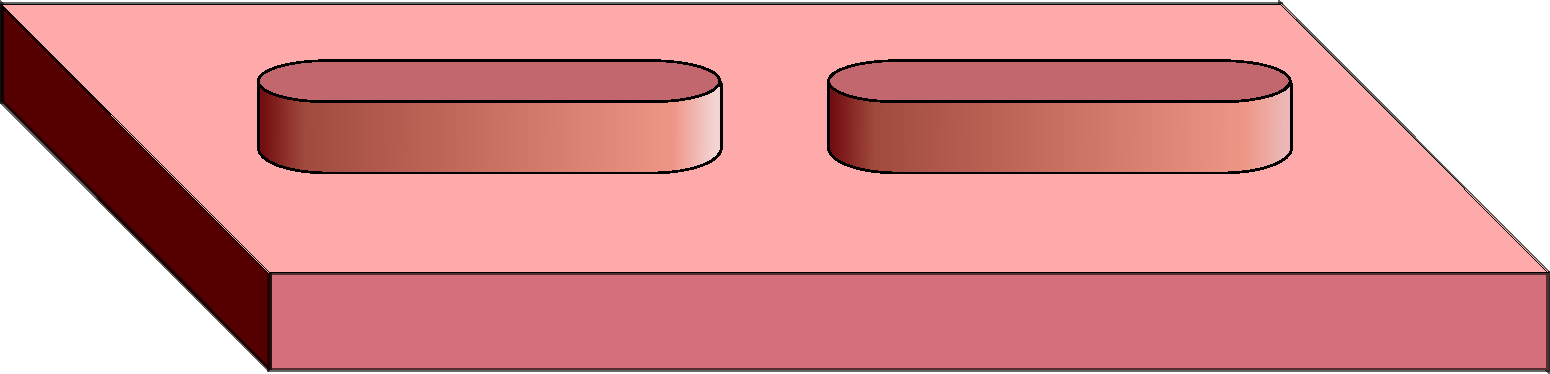
\includegraphics[width = 1.9in]{pill.pdf}
  \label{fig:pill}} \hfil
  \subfloat[]{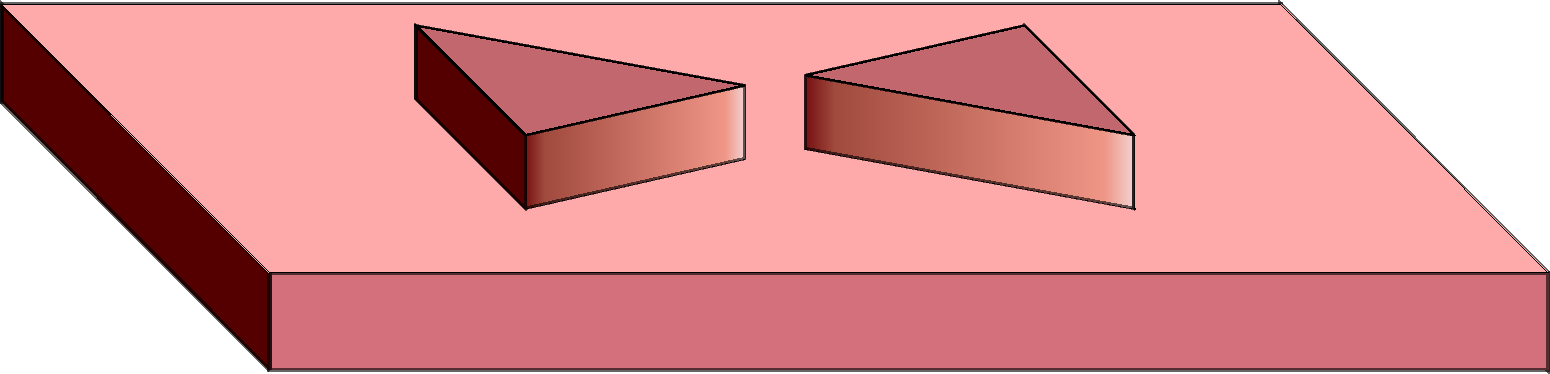
\includegraphics[width = 1.9in]{bowtie.pdf}
  \label{fig:bowtie}} \hfil
  \subfloat[]{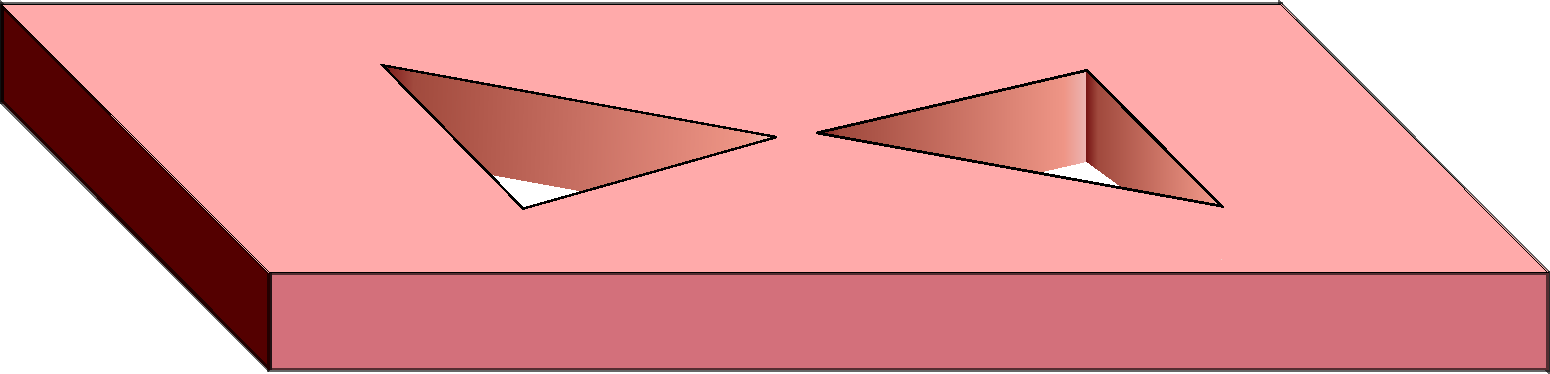
\includegraphics[width = 1.9in]{complementary_bowtie.pdf}
  \label{fig:cbowtie}}
  \caption{Common nanoantenna elements (a) dipole (b) bowtie and (c) aperture. The dipole, bowtie, and aperture antennas are typically etched on a low-loss substrate such as silicon dioxide.}
  \label{fig:antennas}
\end{figure}
%
% Fig. 1 Common nanoantenna elements (a) dipole (b) bowtie (c) aperture and (d) sphere. The dipole, bowtie, and aperture antennas are typically etched on a low loss substrate such as silicon dioxide while spheres may be mounted at the tip of a cone shaped substrate or arranged in some fashion on a flat substrate.
A majority of current research papers focus on free-space designs, but for most practical applications, nanoantennas will be etched on a substrate. The type of substrate depends on the particular application, to some extent determined by the mechanism used to excite the antenna, but for many industrial applications, cost and availability considerations have driven the move to silicon dioxide \ch{SiO2}, often described in technical papers simply as `glass'. Typical signal generation is via off-board laser light or by an on-board transmission line. Unlike classical antenna signals which can be generated at virtually any microwave carrier frequency, there are a select few frequencies where low-cost optical sources are available, although specialized lasers can operate at frequencies throughout the optical spectrum. In optical terminology the signal has traditionally been specified in wavelengths rather than frequency, however here both terms will be used. Some common wavelengths where research is being carried out are in the neighborhood of
\SI{550}, \SI{630}, and \SI{820}{\nm}. An extensive list of various laser types along with their operating frequencies can be found \cite{Weber2000}.
%
% In the optical realm, in addition to referring to `wavelength' rather than `frequency', other commonly encountered terms can at first seem odd or even incorrect to someone accustomed to working in the classical microwave domain. The term `antenna' itself is generally associated with the radiator or receiver component of a circuit, but in the nanometer regime it is also often used when describing a resonator, a device that is not intended for transmission or reception of signals. Also, the term `field intensity' is usually associated with the electric or magnetic field intensity in a microwave system, but in optics it is used to describe what an antenna engineer would refer to as the  `radiation intensity', which is power density multiplied by $r^2$.

A counter-intuitive oddity of noble metals at optical frequencies is that they are no longer perfect conductors, but rather they have some of the properties of a dielectric with, as mentioned above, a permittivity whose real part is negative. This turns out to be a remarkable advantage over dielectrics with a positive real part, due to the fact that the wavelength of the current in these metals can be much less than the wavelength of the free-space incident field. A solid nanorod still resonates around one-half wavelength of its surface current but, given an incident field frequency, one must use numerical or approximate analytical methods to determine the shorter than free-space wavelength of the antenna at resonance. While optical antennas make excellent resonators, due in part to a tightly bound plasmon current, the wavelength mismatch between air and metal, which does not exist at microwave frequencies, is a significant factor hampering their radiation and receiving properties. To understand how the radiation efficiency of an optical antenna can be improved, it is necessary to first study the unusual properties of waves on metals at optical frequencies. The essentials of optical wave propagation and radiation are presented in the following section.
%%%%%%%%%%%%%%%
%%%%%%%%%%%%%%%
%%%%%%%%%%%%%%%
\section{Electromagnetic Theory of Surface Plasmon Polaritons}
%
The physical mechanism for wave propagation at optical frequencies is very different from that of propagating waves at microwave frequencies although the mathematics for determining the wave behavior is virtually the same and can be laid out in a classical Sommerfeld integral analysis. At optical frequencies surface plasmon polaritons (SPPs), electromagnetic surface waves created by coherent charge oscillations in an electron gas in a metal, propagate at a metal-dielectric interface \cite{Ritchie1957,otto1976spectroscopy, Raether1988}. Resonant plasmonic oscillations can also occur in the confined space of nanoparticles \cite{Nie1997}. Fortunately, in most cases where optical antennas are concerned, the quantum mechanisms which create SPPs or local confined plasmons can be expressed in terms of the material properties of metals and nanoparticles, such as shape, size and permittivity \cite{Kelly2003}. Because the study of nanoantennas relies on the behavior of
plasmonic waves, it resides in the research area described as `plasmonics', a
subfield of nanophotonics \cite{Maier2005, Park2009}. In this section, some of the basic theory of SPPs will be presented to aid the reader in understanding the underlying principles that determine the behavior of nanoantennas. First, the fundamental problem of electromagnetic propagation on a planar dielectric-metal interface at optical frequencies is considered, followed by a discussion on the role played by quantum effects in determining the allowable frequency range and loss mechanisms in nano-device design. This presentation does not require an understanding of quantum mechanics, but occasionally the quantum electronics terminologies are used to describe the effects that determine the properties of the constitutive parameters at optical frequencies.
%
%
%
%
\subsection{Single Boundary Structure}
%
Assuming a metal can have a complex permittivity at optical wavelengths, the propagation constants $k_{xi}$ and $k_{zi}$ at the planar interface between dielectric and metal half-spaces, $i = 1,2$ respectively, can be found starting with expressions for transverse magnetic (TM) plane waves in these two regions as shown in Fig. \ref{fig:half_space}. The electromagnetic field expressions in region 1 where $z \ge 0$ are,
%
\begin{subequations}
  \begin{align}
    \v E_1 ={}& \left(\v{\^{x}} E_{x1}  + \v{\^{z}} E_{z1}  \right) \, \e^{ - \j \left(k_x x \,+\, k_{z1} z \right)},
    \label{eq:E_1} \\
    \v H_1 ={}& \v{\^{y}} H_{y1}  \, \e^{ - \j \left(k_x x \,+\, k_{z1} z \right)}
    \label{eq:H_1}
  \end{align}
  \label{eq:field1}%
\end{subequations}
%
\begin{figure}[t!]
  \centering
  \def\svgwidth{.75\linewidth}
  \input{figures/interface.pdf_tex}
  \caption{Dielectric and metal half-spaces with a planar boundary.}
  \label{fig:half_space}
\end{figure}
%
% Fig. 2 Dielectric and metal half-spaces with a planar boundary.
%
and in region 2 where $z \le 0$,
%
\begin{subequations}
  \begin{align}
    \v E_2 ={}& \left(\v{\^{x}} E_{x2}  + \v{\^{z}} E_{z2}  \right) \, \e^{ - \j \left(k_x x \,-\, k_{z2} z \right)},
    \label{eq:E_2} \\
    \v H_2 ={}& \v{\^{y}} H_{y2}  \, \e^{ - \j \left(k_x x \,-\, k_{z1} z \right)}.
    \label{eq:H_2}
  \end{align}
  \label{eq:field2}%
\end{subequations}
%
A positive sign is chosen for $k_{z2}$ to ensure propagation in the negative z direction. The $\Im(k_z)$ must therefore be negative in order to be bounded at infinity.

Ampere's law, $ \del\x{\v H} = -\j \O \E \,\v{E}$, applied to \eqref{eq:field1} and \eqref{eq:field2} yields the boundary conditions:
%
\begin{subequations}
  \begin{align}
    k_{z1} H_{y1} ={}& \O \E_1 E_{x1}
    \label{eq:bc1} \\
    k_{z2} H_{y2} ={}& -\O \E_2 E_{x2}
    \label{eq:bc2}
  \end{align}
  \label{eq:BC}%
\end{subequations}
%
where $\E_{1,2}$ are the permittivities of the dielectric and metal regions respectively. Since metal at optical frequencies has the behavior of a lossy dielectric, continuity of tangential electric and magnetic fields, $E_{x1} = E_{x2}$ and $H_{y1} = H_{y2}$, can be applied at the boundary along with \eqref{eq:BC}. This gives the dispersion relation for waves on the metal-air boundary:
%
\begin{equation}
  \frac{k_{z1}}{\E_1} + \frac{k_{z2}}{\E_2} = 0.
  \label{eq:dispersion}
\end{equation}
%
Helmholtz equation, $\del^2 \v E + k_i^2 \v E = 0$, where $i = 1,2$, and assuming the permeabilities of all regions are that of air, lead to the dispersion equations for the two regions,
%
\begin{equation}
  k_x^2 + k_{zi}^2 = \E_i \left( \frac{\O}{c} \right)^2 = \E_i k_0^2
  \label{eq:ks}
\end{equation}
%
where $c$ is the speed of light in air. Equations \eqref{eq:dispersion} and \eqref{eq:ks} are combined to produce the SPP propagation constant:
%
\begin{equation}
  k_x = k_0 \sqrt{\frac{\E_{r1} \E_{r2}}{\E_{r1} + \E_{r2}}}
  \label{eq:spp}
\end{equation}
%
where $k_0$ is the free-space wavenumber and the subscript $r$ is used to indicate a dielectric constant quantity. If the permittivity of the dielectric is real and that of the metal is complex, $\E_2 = \E_2' - \j \E_2''$, and $\left|\E_2' \right| \gg \E_2''$  the complex propagation constant in \eqref{eq:spp} can be expressed as \cite{Raether1988}:
%
\begin{equation}
  k_x = k_0 \left( \frac{\E_1 \E_2'}{\E_1 + \E_2'} \right)^{1/2} - \j k_0 \, \frac{\E_2''}{2 \,\E_2'^2} \left( \frac{ \E_1 \E_2'}{\E_1 + \E_2'} \right)^{3/2} = k_x' - \j k_x''.
  \label{eq:complec_kx}
\end{equation}
%
Similarly, from \eqref{eq:ks} and \eqref{eq:spp}, $k_{zi}$ becomes approximately,
%
\begin{subequations}
  \begin{align}
    k_{z1} = k_0 \left( \frac{\E_1^2}{\E_1 + \E_2'} \right)^{1/2} + \j k_0 \,  \frac{ \E_1 \E_2''}{2 \left( \E_1 + \E_2' \right)^{3/2}} = k_{z1}' + \j k_{z1}'',
    \label{eq:kz1} \\
    k_{z2} = k_0 \left( \frac{\E_2'^2}{\E_1 + \E_2'} \right)^{1/2} - \j k_0 \, \frac{\E_2''\left( 2\E_1 + \E_2' \right) }{2 \left( \E_1 + \E_2' \right)^{3/2}} = k_{z2}' - \j k_{z2}''.
    \label{eq:kz2}
  \end{align}
  \label{eq:kz}%
\end{subequations}
%
From \eqref{eq:dispersion}-\eqref{eq:kz}, some very important conclusions can be drawn regarding the nature of the two half-space materials and the properties of nano surface waves on their intersecting boundary:
%
\begin{figure}[b!]
  \centering
  \def\svgwidth{.75\linewidth}
  \input{figures/spp.pdf_tex}
  \caption{Surface plasmon propagation along a dielectric-metal boundary and exponential decay perpendicular to the boundary.}
  \label{fig:spp}
\end{figure}
% Fig. 3 Surface plasmon propagation along a dielectric-metal boundary and exponential decay perpendicular to the boundary.
%
\begin{enumerate}
  %
  \item First, if loss is neglected $(\E_2'' \simeq 0)$, a valid assumption for noble metals over significant segments of the optical range so that the permittivities of both regions are real, the equality in \eqref{eq:dispersion} will not hold if these permittivities are both positive or both negative. But, if the permittivity in the dielectric region $1$ is positive, $\E_1 > 0$, and the real part of the permittivity in the metal region $2$ is negative, $\E_2' < 0$, then it is possible to satisfy \eqref{eq:dispersion}.
  %
  \item	Nevertheless, a wave still cannot exist if the term under the square root in \eqref{eq:spp} is negative because this would lead to a totally complex $k_x$, which would mean the fields in \eqref{eq:field1} and \eqref{eq:field2} will exponentially grow or decay rather than propagate along the boundary. However, if
  %
  \begin{equation}
    \E_1 > 0, \quad		 \E_2' < 0, \quad   \text{and}  \quad \left| \E_2' \right| > \E_1,
    \label{eq:conditions}
  \end{equation}
  %
  then the term under the square root in \eqref{eq:spp} is positive and propagation of a wave at the boundary is assured. This condition \eqref{eq:conditions} causes the signs of the terms under the square roots in \eqref{eq:kz} to be negative, but \eqref{eq:dispersion} will still hold as long as same sign for $\sqrt{-1}$ is chosen for both square roots.
  %
  \item	If the conditions in \eqref{eq:conditions} are met then from \eqref{eq:spp}, $k_x > k_0$ and therefore $k_z$ in \eqref{eq:ks} must be complex. According to \eqref{eq:field1} and \eqref{eq:field2}, this results in exponential decay of the field away from the boundary in both the positive and negative z-directions as long as $\sqrt{-1} = -\j$ is chosen for the square root terms in \eqref{eq:kz}. Exponential decay of the plasmon surface wave into the dielectric and metal is illustrated in Fig. \ref{fig:spp}.
  %
  \item	According to Snell's law, the component of the wavenumber $k_x$ tangential to the boundary is the same in both mediums. If medium 1 is air, the x-component of a plane wave incident upon the boundary at an angle $\theta$ from normal is $k_{x1} = k_0 \sin \theta$, which is less than $k_0$. However, according to \eqref{eq:spp} and \eqref{eq:conditions} surface plasmons cannot exist unless $k_x > k_0$. Therefore, surface plasmons cannot be excited by shining light on a flat metal surface.
  %
  \item	From \eqref{eq:complec_kx}, the velocity of a surface plasmon wave on a planar boundary is:
  %
  \begin{equation}
    v_{sp} = \frac{\O}{k_x'} = c \left( \frac{\E_1 + \E_2'}{\E_1 \E_2'} \right)^{1/2}
    \label{eq:velocity}
  \end{equation}
  %
  and its wavelength is:
  %
  \begin{equation}
    \lambda_{sp} = \frac{2 \pi}{k_x'} = \left( \frac{\E_1 + \E_2'}{\E_1 \E_2'} \right)^{1/2}
    \label{eq:wavelength}
  \end{equation}
  %
  \item	The exponential decay of a plasmon along its propagation direction is determined by the second term in \eqref{eq:complec_kx}. The `propagation length' of a plasmon wave is the distance $x = L$ at which the wave decays to   $1/e$ of its initial value. The plasmon propagation length on a planar surface is therefore:
  %
  \begin{equation}
    L = \frac{1}{k_x'} = \frac{2 \,\E_2'^2}{k_0 \,\E_2''} \left( \frac{\E_1 + \E_2'}{\E_1 \E_2'} \right)^{1/2}
    \label{eq:plength}
  \end{equation}
  %
  \item	If the conditions in \eqref{eq:conditions} hold, the second term on the right hand side in \eqref{eq:kz1} and \eqref{eq:kz2} are small so, neglecting these terms, perpendicular to the boundary the $1/e$ decay distance into the dielectric is \cite{Raether1988}:
  %
  \begin{equation}
    z_1 = \left| \frac{1}{k_{z1}'} \right| = \frac{1}{k_0} \left| \frac{2 \, (\E_2')^2}{k_0 \,\E_2''} \left( \frac{\E_1 + \E_2'}{\E_1^2} \right)^{1/2} \right|
    \label{eq:decay_dielectric}
  \end{equation}
  %
  and,
  \begin{equation}
    z_2 = \left| \frac{1}{k_{z2}'} \right| = \frac{1}{k_0} \left| \frac{2 \, (\E_2')^2}{k_0 \,\E_2''} \left( \frac{\E_1 + \E_2'}{\E_2'^2} \right)^{1/2} \right|
    \label{eq:decay_metal}
  \end{equation}
  %
  into the metal.
  \item	Power and energy relationships can be found by assuming a value for the magnetic field amplitude and by using Ampere's law to determine the electric field.
\end{enumerate}
%
The conditions described in \eqref{eq:conditions} are met by noble metals in air for the optical and near-infrared ranges in the case of a TM polarized wave. A similar analysis will show that a transverse electric (TE) polarized wave cannot exist at a dielectric-metal boundary.

In practical applications, one should take care in the selection of the metal to be used in a nanoantenna design. Some metals, such as silver, tend to develop an oxidation layer, which can severely decrease propagation length and increase the antenna impedance. For a more detailed discussion concerning the effect of a silver sulfide oxidation layer on a silver substrate plasmon wave, the reader is referred to \cite{Nevels2014}.
%
Fig. \ref{fig:plength} shows the propagation length as a function of wavelength for three metals, gold, silver and aluminum \cite{9783540339199}. The practitioner is cautioned that although the propagation length of a surface plasmon does increase as frequency decreases, the analysis leading to this figure is based on an idealization of the physical problem. Here, a pure wave propagation condition was assumed in the formulation of equations \eqref{eq:field1} and \eqref{eq:field2}. In the practical case, a source such as the feed point of an antenna, must be included in the problem formulation. If the source is included, one sees that as the frequency decreases, less energy is transferred into the surface plasmon wave and more into the space wave; the field that is radiated directly into space from the source point. In the far infrared frequency range, the surface plasmon essentially ceases to exist. Plasmon wave behavior is discussed in more detail in the section of this chapter concerning aperture antennas.
%
\begin{figure}[t!]
  \centering
  {\includegraphics[width = .5\linewidth]{generate_fig4.tikz}}
  \caption{Propagation length of a surface plasmon propagating along the interface between a dielectric (refractive index 1.32) and a metal as a function of wavelength calculated for gold (Au), silver (Ag), and aluminum (Al).}
  \label{fig:plength}
\end{figure}
% Fig. 4 Propagation length of a surface plasmon propagating along the interface between a dielectric (refractive index 1.32) and a metal as a function of wavelength calculated for gold (Au), silver (Ag), and aluminum (Al).
%
%%%%%%%%%%%%%%%
%%%%%%%%%%%%%%%
%%%%%%%%%%%%%%%
\section{Quantum effects}
%
The above analysis considers only the classical electromagnetic aspects of propagation on a dielectric metal boundary. However, quantum mechanical effects inherent in metals and dielectrics enter the picture through the permittivity, thereby determining its value as well as the frequency range over which SPPs can propagate. Essentially, quantum processes reveal the frequency range over which the metal has a permittivity with a negative real part and where losses begin to have a serious effect on wave propagation within that frequency range. In the following, the influence of plasma resonance and atomic collisions on SPP propagation are briefly explored.  Although the properties described below are best understood using quantum mechanics, the mathematics below is classical, primarily developed by concatenating harmonic oscillator models. However, the differences in the results of the two theories is small, allowing classical electromagnetic calculations without the necessity of delving into quantum theory.
Free electrons can exist near the top of the energy band distribution in a metal. The interaction of these electrons with photons and the long-range Coulomb force of atoms create an electron oscillation known as a plasmon. Taking these effects into account, the dielectric function of metal can be expressed in terms of the Drude model \cite{MaxBorn2002}:
%
\begin{equation}
  \E(\O) = 1 - \frac{\O_p^2}{\O(\O  - \j \nu)} = \left(1 - \frac{\O_p^2}{\O^2 + \nu^2} \right) - \j \frac{\nu \, \O_p^2}{\O (\O^2 + \nu^2)} = \E_r - \j \E_i
  \label{eq:drude}
\end{equation}
%
where $\nu = 1/\tau$ is the collision frequency, $\tau$ is the scattering time between collisions, and $\O_p$ is the plasma frequency that is expressed as:
%
\begin{equation}
  \O_p = \sqrt{\frac{N e^2}{\E_0 m_e}}
  \label{eq:plasma_f}
\end{equation}
%
in which $e$ and $m_e$ are the electron charge and mass respectively and $N$ is the concentration of free electrons. Plasma frequencies for metals are in the visible and ultraviolet ranges. Typical values of plasma and collision frequencies are $\O_p = \SI{.23e12}{\Hz}$ and
$\nu = \SI{5.51e12}{\Hz}$ for gold and $\O_p = \SI{.21e16}{\Hz}$ and $\nu = \SI{4.45e12}{\Hz}$ for silver, however impurities and other factors can affect these numbers so the literature does not have a unique set of values for these parameters. A comprehensive list of plasma and collision frequencies published by a variety of researchers for gold, silver and other noble metals can be found at \cite{Moroz2010}.

Collisions are primarily between electrons and relatively large lattice vibrations (phonons), so for most metals at room temperature  $\nu \ll \O_p $ \cite{Bohren1998}, which reduces \eqref{eq:drude} to approximately:
%
\begin{equation}
  \E(\O) \simeq 1 - \frac{\O_p^2}{\O^2}
  \label{eq:drude_approx}
\end{equation}
%
This important expression shows that when $\O < \O_p$, then $\E(\O) < 0$  which in part satisfies the conditions in \eqref{eq:conditions}. Therefore, surface plasmon polaritons can only exist below the plasma frequency. Equation \eqref{eq:drude_approx} substituted into \eqref{eq:spp} gives a simplified Drude model for the plasmon wavenumber:
%
\begin{equation}
  k_x \simeq k_1 \left( \frac{\O^2 - \O_p^2}{\O^2 \E_{r1} + (\O^2 - \O_p^2)} \right)^{1/2}
  \label{eq:kx_approx}
\end{equation}
%

The Drude model in the form given in \eqref{eq:drude} is widely used in nanoantenna analytical and numerical calculations for determining the permittivity, and therefore the propagation constant, of the plasmon polariton of noble metals. However, this free electron model fails at frequencies higher than about \SI{850}{\tera\Hz} \cite{Archambault2009}, due to bound charge effects, and must be modified by incorporating additional terms \cite{Bohren1998}. This becomes a tedious process but reasonable accuracy can be achieved. Another option, preferred by the authors, is to use measured data \cite{Lynch1997} with a partial fraction fit \cite{Michalski2013}. Fig. \ref{fig:permittivity} shows the dielectric function for gold and silver over the frequency range from \SI{.5}{\electronvolt}\texttildelow \SI{120}{\THz} to \SI{6.5}{\electronvolt}\texttildelow \SI{1.57}{\peta \Hz} obtained from measured data via a partial fraction fit. The solid lines are the
partial fraction fit for the real part $\E'$, and the dashed lines are for the imaginary part $\E''$, of the dielectric function.
%
\begin{figure}[t!]
  \centering
  \subfloat[]{\includegraphics[width = .5\linewidth]{ep_gold.tikz}
  \label{fig:ep_gold}} \\
  \subfloat[]{\includegraphics[width = .5\linewidth]{ep_silver.tikz}
  \label{fig:ep_silver}}
  \caption{Dielectric function for (a) Gold and (b) Silver as a function of  photon energy $E = hf$ where $f$ is frequency and $h = \SI{6.626e34} {kg.m^{2}/s}$ is Planck's constant. The solid lines are the partial fraction fit for $\E'$ and the dashed line is for $\E''$. The circles and squares are from measured data originally listed in \cite{Johnson1972}}
  \label{fig:permittivity}
\end{figure}
% Fig. 5 Dielectric function for (a) Silver and (b) Gold as a function of photon energy where f is frequency and   m2 kg/s is Planck's constant. The solid lines are the partial fraction fit for  and the dashed line is for   . The circles and squares are from measured data originally supplied by (Johnson and Christy 1972).
%

The significance of the data in Fig. \ref{fig:permittivity} becomes clearer in Fig. \ref{fig:dispersion} where the surface plasmon dispersion curve for frequency versus the propagation $k_x'$, attenuation $k_x''$, and constants at an air-silver boundary are plotted. The lower part of the curve is the non-radiative surface plasmon region followed above by an anomalous dispersion region and above that a Brewster mode radiative region. The slanted dashed line is the free-space light line $k_0 = \O/c$. The Brewster mode portion of the dispersion curve is in the fast wave region to the left of the light line. It is the locus of the values of $k_x$ of the plane wave incident on the boundary at the Brewster angle. These waves do not set up a surface wave, but rather carry their power directly into the metal without reflection. Below the Brewster mode section is a region of anomalous dispersion, often described in the literature as `backbending', which has a group velocity that is virtually zero, and is accompanied by high loss.
%
\begin{figure}[t!]
  \centering
  {\includegraphics[width = .5\linewidth]{disp_silver.tikz}}
  \caption{SPP dispersion curve for $\O$ versus $\Re (k_x)$ and $\Im (k_x)$ for an glass-silver interface. The lower part of the curve is the non-radiative surface plasmon region which is capped by a high-loss backbending region, and a Brewster mode radiative region above}
  \label{fig:dispersion}
\end{figure}
% Fig. 6 SPP dispersion curve for   versus   and   for an air-silver interface. The lower part of the curve is the non-radiative surface plasmon region which is capped by a high loss backbending region, and a Brewster mode radiative region above.
%

The surface plasmon portion of the dispersion curve is of primary importance to nanoantenna design. The plasmon region lies to the right of the light line and therefore, it is a slow wave since the phase velocity here is less than the speed of light. Because surface plasmons have a shorter wavelength than light they are prevented from radiating from a flat planar surface. Of particular significance is the decreasing slope of the dispersion curve, tending toward horizontal near where it joins the anomalous dispersion segment. In the plasmon region the surface plasmon propagation constant increases dramatically with a small increase in frequency. The horizontal dashed line at \SI{380}{\nm} intersects the light line at approximately $k_0 = \SI{17}{\radian \per \micm}$ while at the same wavelength $k_x' = \SI{21}{\radian \per \micm}$, which means the surface plasmon wavelength can be much less than the free-space wavelength. Therefore, a resonant half-wavelength nano-dipole antenna can be much smaller than a half-wavelength measured in air at the same frequency. As the plasmon wavelength decreases near the anomalous dispersion region, the propagation constant approaches a limiting value. The Drude model provides the estimate for this limiting frequency
%
\begin{equation}
  \O_{sp} \simeq \O_p/\sqrt{1 + \E_{r1}},
  \label{eq:apprx_plasma_freq}
\end{equation}
%
obtained by setting the denominator in \eqref{eq:kx_approx} equal to zero, which is equivalent to assuming the propagation constant in \eqref{eq:kx_approx} approaches infinity. This is not what happens to the propagation constant, as can be seen in Fig. \ref{fig:dispersion} where real data is used, but it does provide a reasonable estimate of the limiting frequency. nanoantennas must be designed to operate below this frequency, thereby avoiding a group velocity approaching zero and dramatically increased losses.

Although several key aspects of wave propagation on nano-structures have been presented here, all analysis has been performed assuming propagation is on a surface between two half spaces. However, most nanoantennas have air above and are etched in a noble metal, such as gold, on a dielectric substrate, such as silicon dioxide. The metal antenna, therefore lies between two different materials. nanoantennas are typically excited at a corner or edge where both upper and lower surfaces are exposed to the incoming electromagnetic field. Because the plasmon propagation constant \eqref{eq:complec_kx} is a function of the permittivity in the regions above and below an interface, it will be helpful to understand how different phase velocities \eqref{eq:velocity} and wavelengths \eqref{eq:wavelength} on the two sides of a nanoantenna will affect its performance. This issue is briefly addressed in the following paragraphs.
%%%%%%%%%%%%%%%
%%%%%%%%%%%%%%%
%%%%%%%%%%%%%%%
%%%%%%%%%%%%%%%
%%%%%%%%%%%%%%%
%%%%%%%%%%%%%%%
\section{Two Boundary Structures}
%
Surface plasmon polaritons on a metal film have properties that do not exist on an interface between metal-dielectric half spaces. To analyze the mode configuration on a metal strip of thickness $t$, consider the configuration shown in Fig. \ref{fig:3layer} where the dielectrics are assumed to extend from the surface of the metal to infinity and possess different permittivities, $\E_1$ and $\E_2$. The permittivity of the metal is $\E_m$ and all three regions have the permeability of free-space. The waves in each region are assumed to be TM polarized with a magnetic field component in the y-direction in each region given by:
%
\begin{figure}[b!]
  \centering
  \def\svgwidth{.75\linewidth}
  \input{figures/three_layer.pdf_tex}
  \caption{Thin metallic film between two dielectric regions with different permittivities.}
  \label{fig:3layer}
\end{figure}
% Fig. 7 Thin metallic film between two dielectric regions with different permittivities.
%
\begin{subequations}
  \begin{align}
    \v H_1 ={}& \v{\^{y}} \,H_{y1} \, \e^{ -\A_{z1}z \,- \j k_x x}, \qquad	 		\text{dielectric region 1} (z \ge t)
    \label{eq:H1_3layer}\\
    \v H_m ={}& \v{\^{y}} \,\left( H_{ya}\, \e^{ +\A_{zm}z} + H_{yb}\, \e^{ -\A_{zm}z} \right) \, \e^{ - \j k_x x}, \qquad	 		\text{metal region m} (0 \le z \le t)
    \label{eq:Hm_3layer}\\
    \v H_2 ={}& \v{\^{y}} \,H_{y2} \, \e^{ -\A_{z3}z \, - \j k_x x}, \qquad	 		\text{dielectric region 2} (z \le 0)
    \label{eq:H2_3layer}
  \end{align}
  \label{eq:H_3layer}%
\end{subequations}
%
where the dispersion relations for the three regions are,
%
\begin{equation}
  \A_{zi}^2 = -k_{zi}^2 = k_x^2 - k_0^2 \E_i, \qquad	  \text{for} \,
  i=1,2,m
  \label{eq:3_layer_disp}
\end{equation}
%
and the boundary conditions satisfied by $\v H_m$ at each interface are:
%
\begin{subequations}
  \begin{align}
    {H_{ym}} ={}& {H_{yi}}
    \label{eq:bc1_3layer}\\
    \frac{1}{\E_m}\pdv{H_{ym}}{z}  ={}& \frac{1}{\E_i}\pdv{H_{yi}}{z}
    \label{eq:bc2_3layer}
  \end{align}
  \label{eq:bc_3layer}%
\end{subequations}
%
where $i = 1,2$. Each of these conditions are applied to \eqref{eq:H_3layer} at each boundary yielding a set of four homogeneous linear equations which can be combined to produce:
%
\begin{subequations}
  \begin{align}
    \frac{H_{yb}}{H_{ya}} ={}& \ddfrac{\left(\frac{\E_2 \,\A_{zm}}{\E_m \,\A_{z2}} - 1 \right)}   {\left(\frac{\E_2 \,\A_{zm}}{\E_m \,\A_{z2}} + 1 \right)}
    \label{eq:homo1_3layer}\\
    \frac{H_{yb} \, \e^{-2 \A_{zm}t}}{H_{ya}} ={}& \ddfrac{\left(\frac{\E_1 \,\A_{zm}}{\E_m \,\A_{z1}} + 1 \right)}   {\left(\frac{\E_1 \,\A_{zm}}{\E_m \,\A_{z1}} - 1 \right)}
    \label{eq:homo2_3layer}
  \end{align}
  \label{eq:homo_3layer}%
\end{subequations}
%
The equations in \eqref{eq:homo_3layer} are equated to produce the three dispersion relation:
%
\begin{equation}
  \left(\frac{\E_m \,\A_{z1}}{\E_1 \,\A_{zm}} + 1 \right) \left(\frac{\E_m \,\A_{z2}}{\E_2 \,\A_{zm}} + 1 \right) = \left(\frac{\E_m \,\A_{z1}}{\E_1 \,\A_{zm}} - 1 \right) \left(\frac{\E_m \,\A_{z2}}{\E_2 \,\A_{zm}} - 1 \right) \, \e^{-2\A_{zm}t}
  \label{eq:3layer_dispersion}
\end{equation}
%
for the metal layer sandwiched between two different dielectrics. Equation \eqref{eq:3layer_dispersion} can be verified by allowing the metal thickness to become large, $\A_{zm}t \rightarrow \inf$, in which case the right hand side goes to zero. This yields a pair of equations:
%
\begin{subequations}
  \begin{align}
    \frac{\E_m \A_{z1}}{\E_1 \,\A_{zm}} + 1 ={}& 0
    \label{eq:simplified1_3layer_to2layer}\\
    \frac{\E_m \A_{z2}}{\E_2 \,\A_{zm}} + 1 ={}& 0,
    \label{eq:simplified2_3layer_to2layer}
  \end{align}
  \label{eq:simplified_3layer_to2layer}%
\end{subequations}
%
recognized from \eqref{eq:dispersion} to be the dispersion relations for surface plasmon polaritons at the boundaries between two individual dielectric-metal half-spaces.

If $\E_1$ and $\E_2$ are positive and $\E_m < 0$, the right hand side of \eqref{eq:3layer_dispersion} is positive, which means the left hand side must also be positive. This is possible if,
$\left( \frac{\E_m \,\A_{z1}}{\E_1 \,\A_{zm}} + 1 \right)$ and
$\left( \frac{\E_m \,\A_{z2}}{\E_2 \,\A_{zm}} + 1 \right)$ are both positive or both negative. Under the assumption that both are negative, that
$ \E_1 > \E_2 $, and $\left| \E_m \right| > \E_1$  the characteristic equation \eqref{eq:3layer_dispersion} becomes \cite{Durach_2007},
%
\begin{equation}
  \A_{zm}t = \coth ^{-1} \left( \frac{\left| \E_m \right|\A_{z1}}{\E_1 \,\A_{zm}} \right) + \coth ^{-1} \left( \frac{\left| \E_m \right|\A_{z2}}{\E_2 \,\A_{zm}} \right).
  \label{eq:3layer_xtic_coth}
\end{equation}
%
Similarly, assuming that both expressions in brackets on the left hand side of \eqref{eq:3layer_dispersion} are positive and
$\left| \E_m  \right| < \frac{\E_1 \E_2}{\E_1 - \E_2}$  the characteristic equation becomes \cite{Durach_2007},
%
\begin{equation}
  \A_{zm} t = \tanh^{-1} \left( \frac{\left| \E_m \right| \A_{z1}}{\E_1 \,\A_{zm}} \right) + \tanh^{-1} \left( \frac{\left| \E_m \right| \A_{z2}}{\E_2 \,\A_{zm}} \right).
  \label{eq:3layer_xtic_tanh}
\end{equation}
%
Equations \eqref{eq:3_layer_disp} together with \eqref{eq:3layer_xtic_coth} or \eqref{eq:3layer_xtic_tanh} can be used to solve for the wavenumbers in the even and odd mode cases, referring respectively to the symmetric or asymmetric form of the tangential (z-directed) component of the electric field about the center of the metal layer \cite{Burke1986}.

When the metal layer is thick, the waves on the two sides of the metal slab do not interact, as indicated in \eqref{eq:simplified_3layer_to2layer}. However, as the slab becomes thinner the electromagnetic fields on the two sides do interact and the frequency splits into a low frequency even mode \eqref{eq:3layer_xtic_coth} and a higher frequency odd mode \eqref{eq:3layer_xtic_tanh}. Although the tangential electric field is not entirely symmetric in the metal region when $\E_1 \ne \E_2$, more of the field lies inside the metal in the even mode case \eqref{eq:3layer_xtic_coth} than it does in the basically asymmetric odd mode case \eqref{eq:3layer_xtic_tanh}. As the metal layer becomes thinner, the damping of the odd mode decreases, approximately as the square of the thickness, allowing this mode to travel a greater distance than a plasmon polariton on the interface between two half spaces. However, the basically symmetric mode damping increases with decreasing thickness, allowing propagation distances one or two orders of magnitude greater than those of thick metal construction
\cite{Sarid1981}. The physical reason attributed to this phenomena is that in the asymmetric case, where the null is in the center of the metal, more of the field resides outside as the thickness of the metal decreases therefore, lessening the presence of the tangential electric field in the metal thereby reducing Joule heat which in turn decreases the electron collision rate resulting in less damping of the wave. This analysis suggests that the efficiency of an optical antenna can be improved by decreasing the thickness of the metallic material with which it is constructed and operating in the higher odd mode frequency range.

When the metal width is finite and the environment is symmetric $(\E_1 = \E_2)$, there are four fundamental modes and a number of higher order modes. These modes can be classified according to the cross-sectional width and thickness, similar to a rectangular waveguide and will become successively cut off as the thickness decreases leaving one Gaussian like mode. Efficient optical fiber coupling to this plasmonic mode in a metal guide has been demonstrated \cite{Berini2000}, raising the possibility of similar coupling between optical antennas and metal strip plasmonic waveguides designed with the appropriate width and thickness so as to operate in this particular mode. Closer to the nanoantenna case, in an asymmetric environment $(\E_1 \ne \E_2)$ there is no purely TM mode. It has been shown that modes in this case can change their symmetry properties with changes in both transverse directions, width and thickness, and that all modes show a cutoff height that increases both with decreasing width and increasing dielectric mismatch
between the sub- and superstrate \cite{Berini2000,Berini2001}. Unfortunately, this includes air-metal-glass configurations commonly used in the design of optical antennas and waveguides. Thus the complicated spatial profiles shown in modes in an asymmetric environment prohibit efficient excitation techniques \cite{Maier2005,Yang1991}.

In this section it has been shown that in the optical frequency range electromagnetic wave propagation, which is via a surface plasmon polariton, can take place on an air-dielectric boundary if one of the two materials has a dielectric constant with a negative real part obeying the conditions in \eqref{eq:conditions}. The dispersion equation for this wave is given in \eqref{eq:spp} and presented graphically in Fig. \ref{fig:dispersion}, which shows that a surface plasmon is a slow wave, i.e. slower than the speed of light in the dielectric medium. The Drude model, which is relatively accurate below, and not too close to, the plasma frequency $\O_p$ and useful for analytical calculations, was given in \eqref{eq:drude}. This model, or its approximation in \eqref{eq:drude_approx}, is commonly used to obtain approximate velocity \eqref{eq:velocity}, wavelength \eqref{eq:wavelength}, propagation distance \eqref{eq:plength}, and exponential decay distance away from the boundary \eqref{eq:decay_dielectric} and
\eqref{eq:decay_metal} of the plasmon wave. It also provides an estimate of maximum frequency \eqref{eq:apprx_plasma_freq} at which a plasmon wave can propagate. Although Fig. \ref{fig:dispersion} shows that the surface plasmon wavelength can be much less than the free-space wavelength, close to the maximum frequency the plasmon wave will experience severe attenuation.

Because optical antennas are operated in a frequency range which is at the overlapping boundary between electromagnetic and quantum theories, in the paragraphs above, some of the quantum justification for the unusual behavior of materials in the near infrared and optical domains has been presented. This discussion was then followed by an asymmetric two boundary case development of the dispersion equations modeling a typical optical antenna structure in cross-section, showing that the interaction between the plasmon waves on the two boundaries breaks into symmetric and asymmetric modes, \eqref{eq:3layer_xtic_coth} and \eqref{eq:3layer_xtic_tanh}. The symmetric mode is preferred when coupling to another device and the asymmetric mode is preferred for long distance propagation in a plasmon waveguide. This section then concluded with a discussion of the finite width metal guide that has been shown to have a complicated mode structure, hampering efforts to obtain a mathematical expression for impedance matching. Current attempts at obtaining a mathematical model and along with design methods that improve impedance matching and enhance optical antenna radiation will be covered in the individual antenna discussions that follow.
%%%%%%%%%%%%%%%
%%%%%%%%%%%%%%%
%%%%%%%%%%%%%%%
%%%%%%%%%%%%%%%
%%%%%%%%%%%%%%%
%%%%%%%%%%%%%%%
\section{Design of Optical Antennas}
%
The plasmonic nature of nanoantenna operation prevents the designer from describing antenna performance with formulas that have been developed over many decades at microwave and lower frequencies. Dielectric properties of metals are only one factor preventing a direct correspondence between established antenna theory and actual optical antenna operation. A traditional antenna concept that the wave vector for the current is the same as the free-space wave vector must be abandoned, dispersion effects must be accounted for and losses not generally expected in a microwave frequency  `perfect conductor' become dependent on the size and shape of the antenna.
The optical antenna, although not a traditional perfect conductor, cannot be analyzed as though it is a pure dielectric rod as would be the case for an optical fiber. But even if an optical antenna could be modeled as a pure dielectric, the tips of a rod represent the famous unsolved dielectric wedge problem. As described above, the fast wave current on a perfect conductor must be replaced by a slow wave plasmon current tightly coupled to the antenna surface. Radiation on an optical dipole still occurs at the tips of the rods and can still be viewed as current induced. The primary difficulty that must be faced when attempting an analytical analysis is that for practical reasons the design requires placing the antenna on an interface between a dielectric below, such as a silicon dioxide substrate, and air above. Although numerical techniques can be used to accurately analyze the characteristics of the structure, similar to microstrip patch antennas, no exact analytical methods are available. Analytical approximations and numerical attempts to obtain the basic characteristics of an optical antenna, the resonant frequency, input impedance, gain, directivity and efficiency, are presented in this section.
%%%
%%%
%%%
\subsection{Dipole and Patch Antennas}
%
Size and shape can affect the design frequency of an optical antenna in ways not typically expected in microwave frequency antenna engineering. For example a rectangular microstrip patch is expected to resonate when the incident field is polarized in the direction of the $\lambda/2$ dimension of the patch, while the transverse dimension is flexibly left to something greater or less than $\lambda/2$. However, as shown in Fig. \ref{fig:simulation} both the width and length of a metal plate must be considered in designing an optical antenna. A narrow nanodipole resonating at a particular frequency, as shown in Fig. \ref{fig:nitin_dipole}, does not maintain resonance
%
\begin{figure}[b!]
  \centering
  \def\svgwidth{.75\linewidth}
  \input{figures/dipoles_nitin.pdf_tex}
  \caption{A gold dipole residing over a glass substrate.}
  \label{fig:nitin_dipole}
\end{figure}
%
\begin{figure}[t!]
  \centering
  \subfloat[]{\includegraphics[height = 2.7in]{generate_fig8c.tikz}
  \label{fig:sim_hi}}\\
  \centering
  \subfloat[]{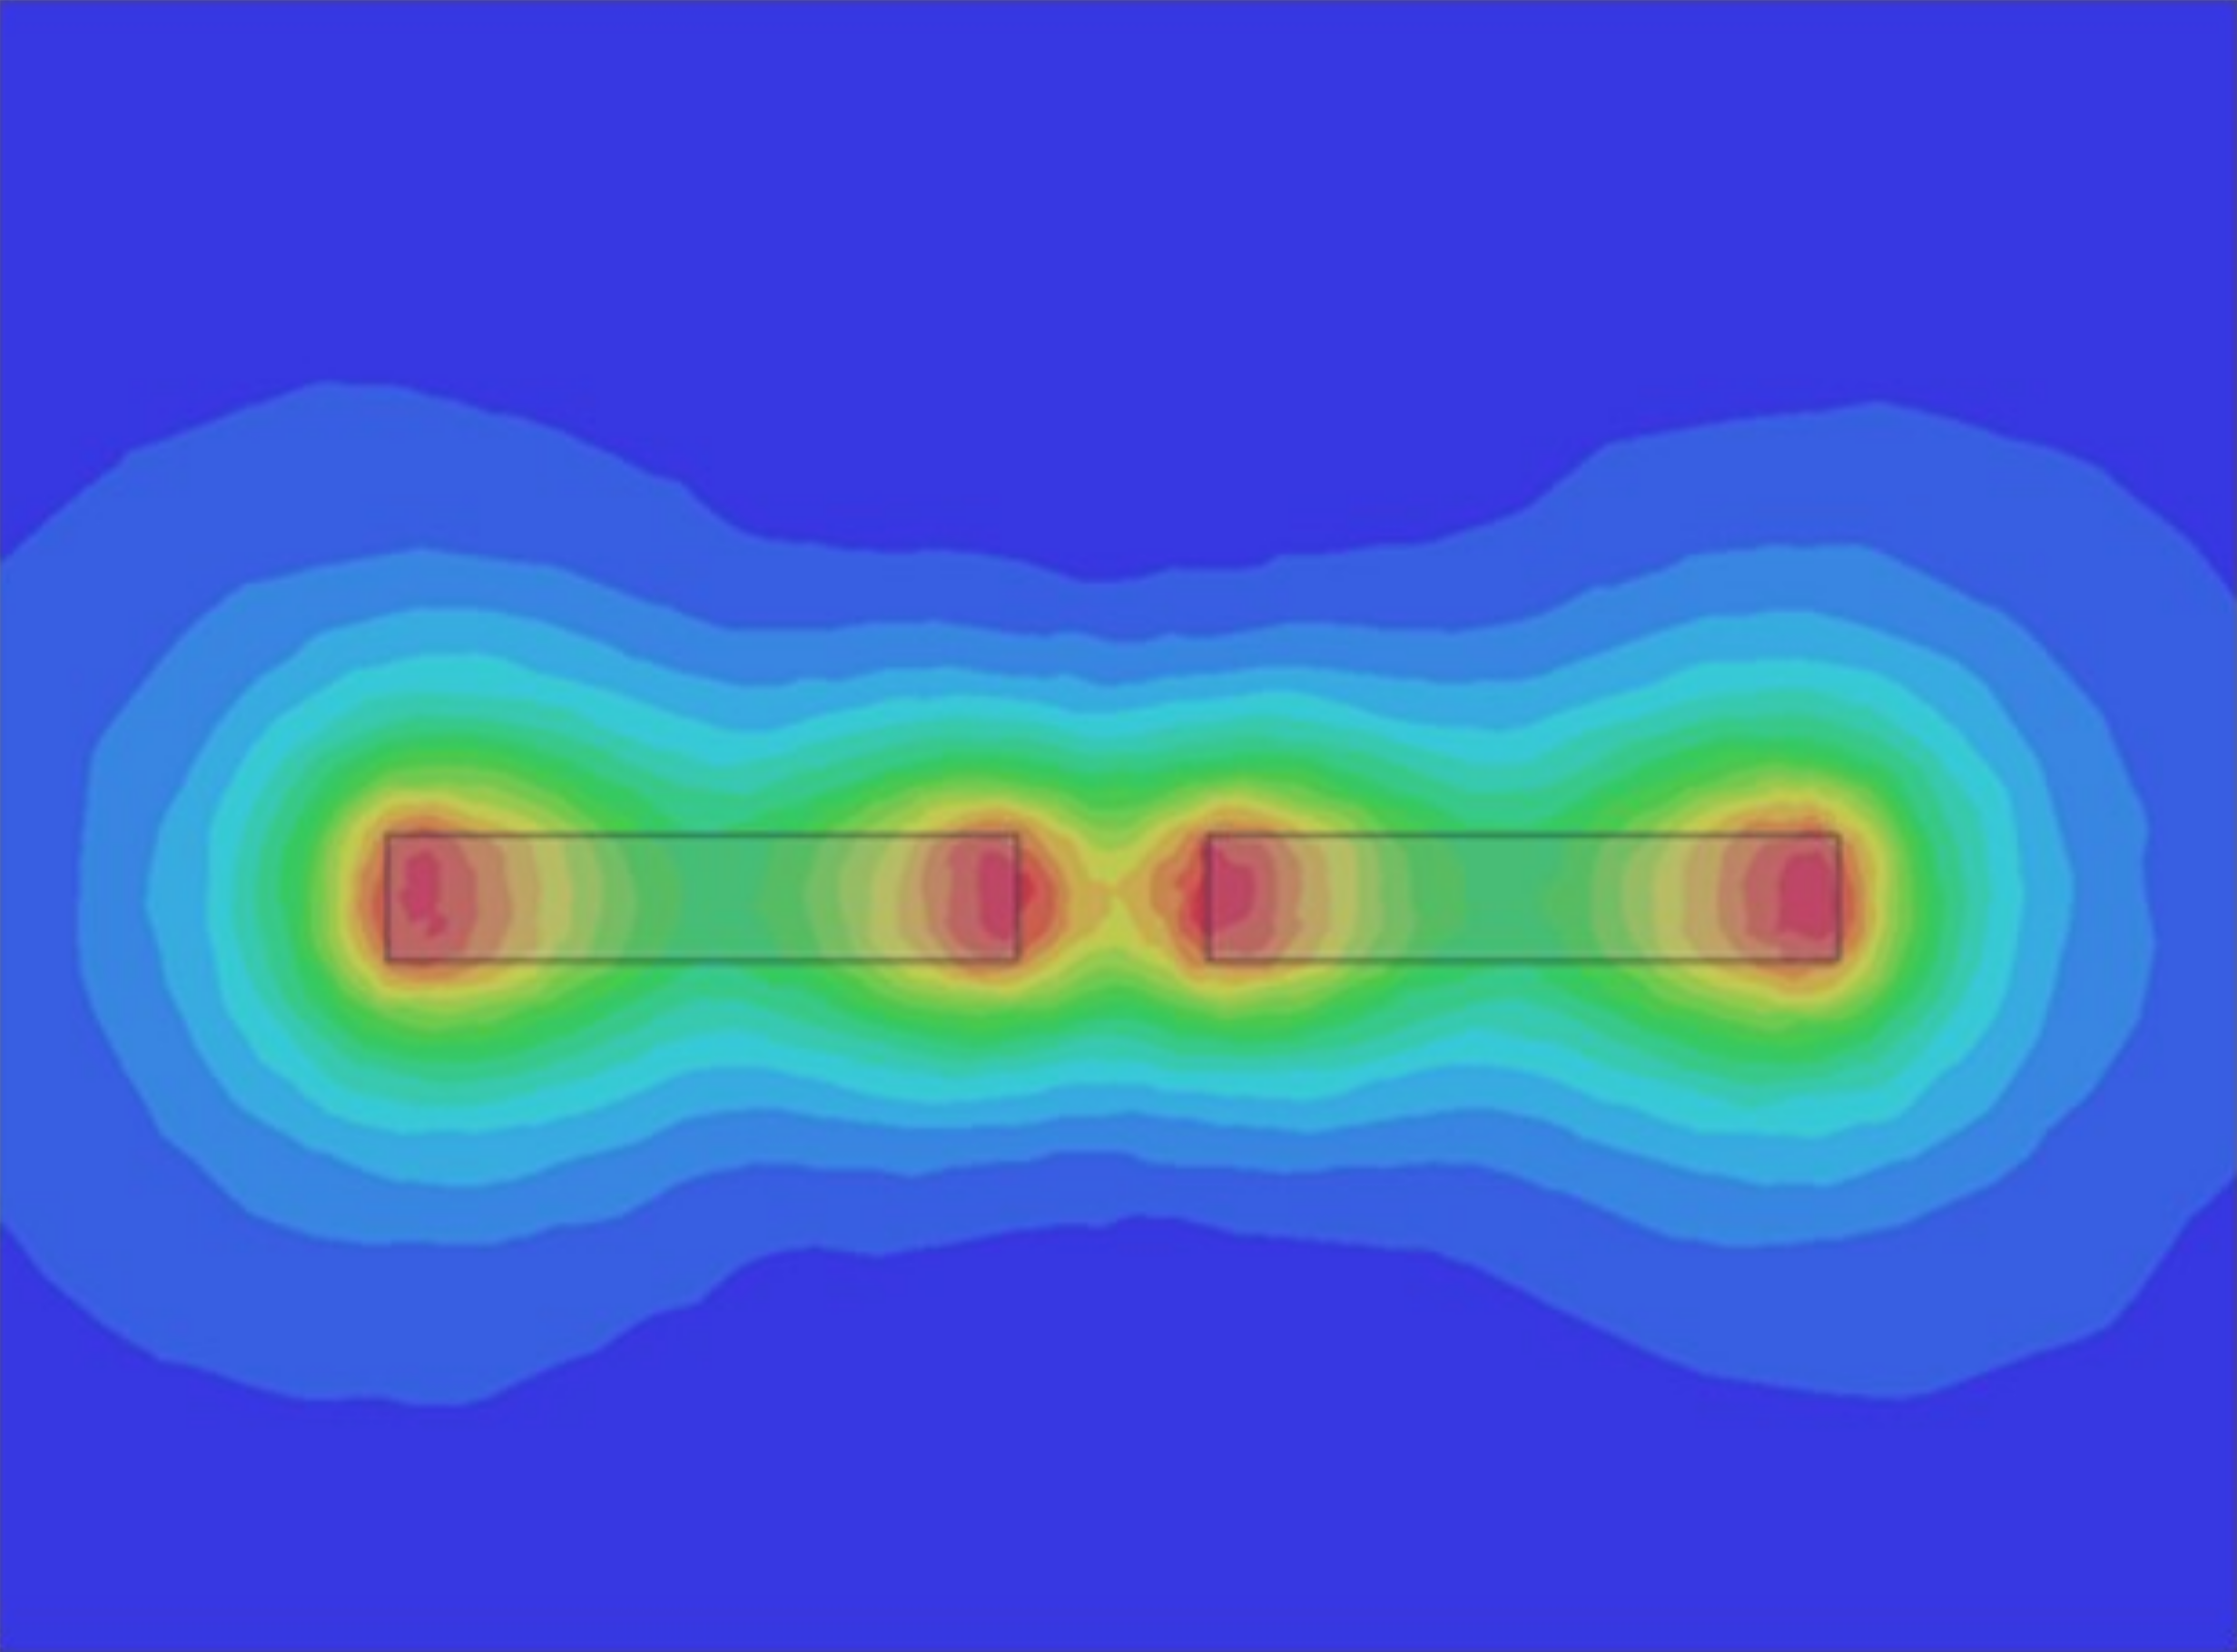
\includegraphics[height = 1.9in]{fig8_a.png}
  \label{fig:narrow}} \hfil
  \subfloat[]{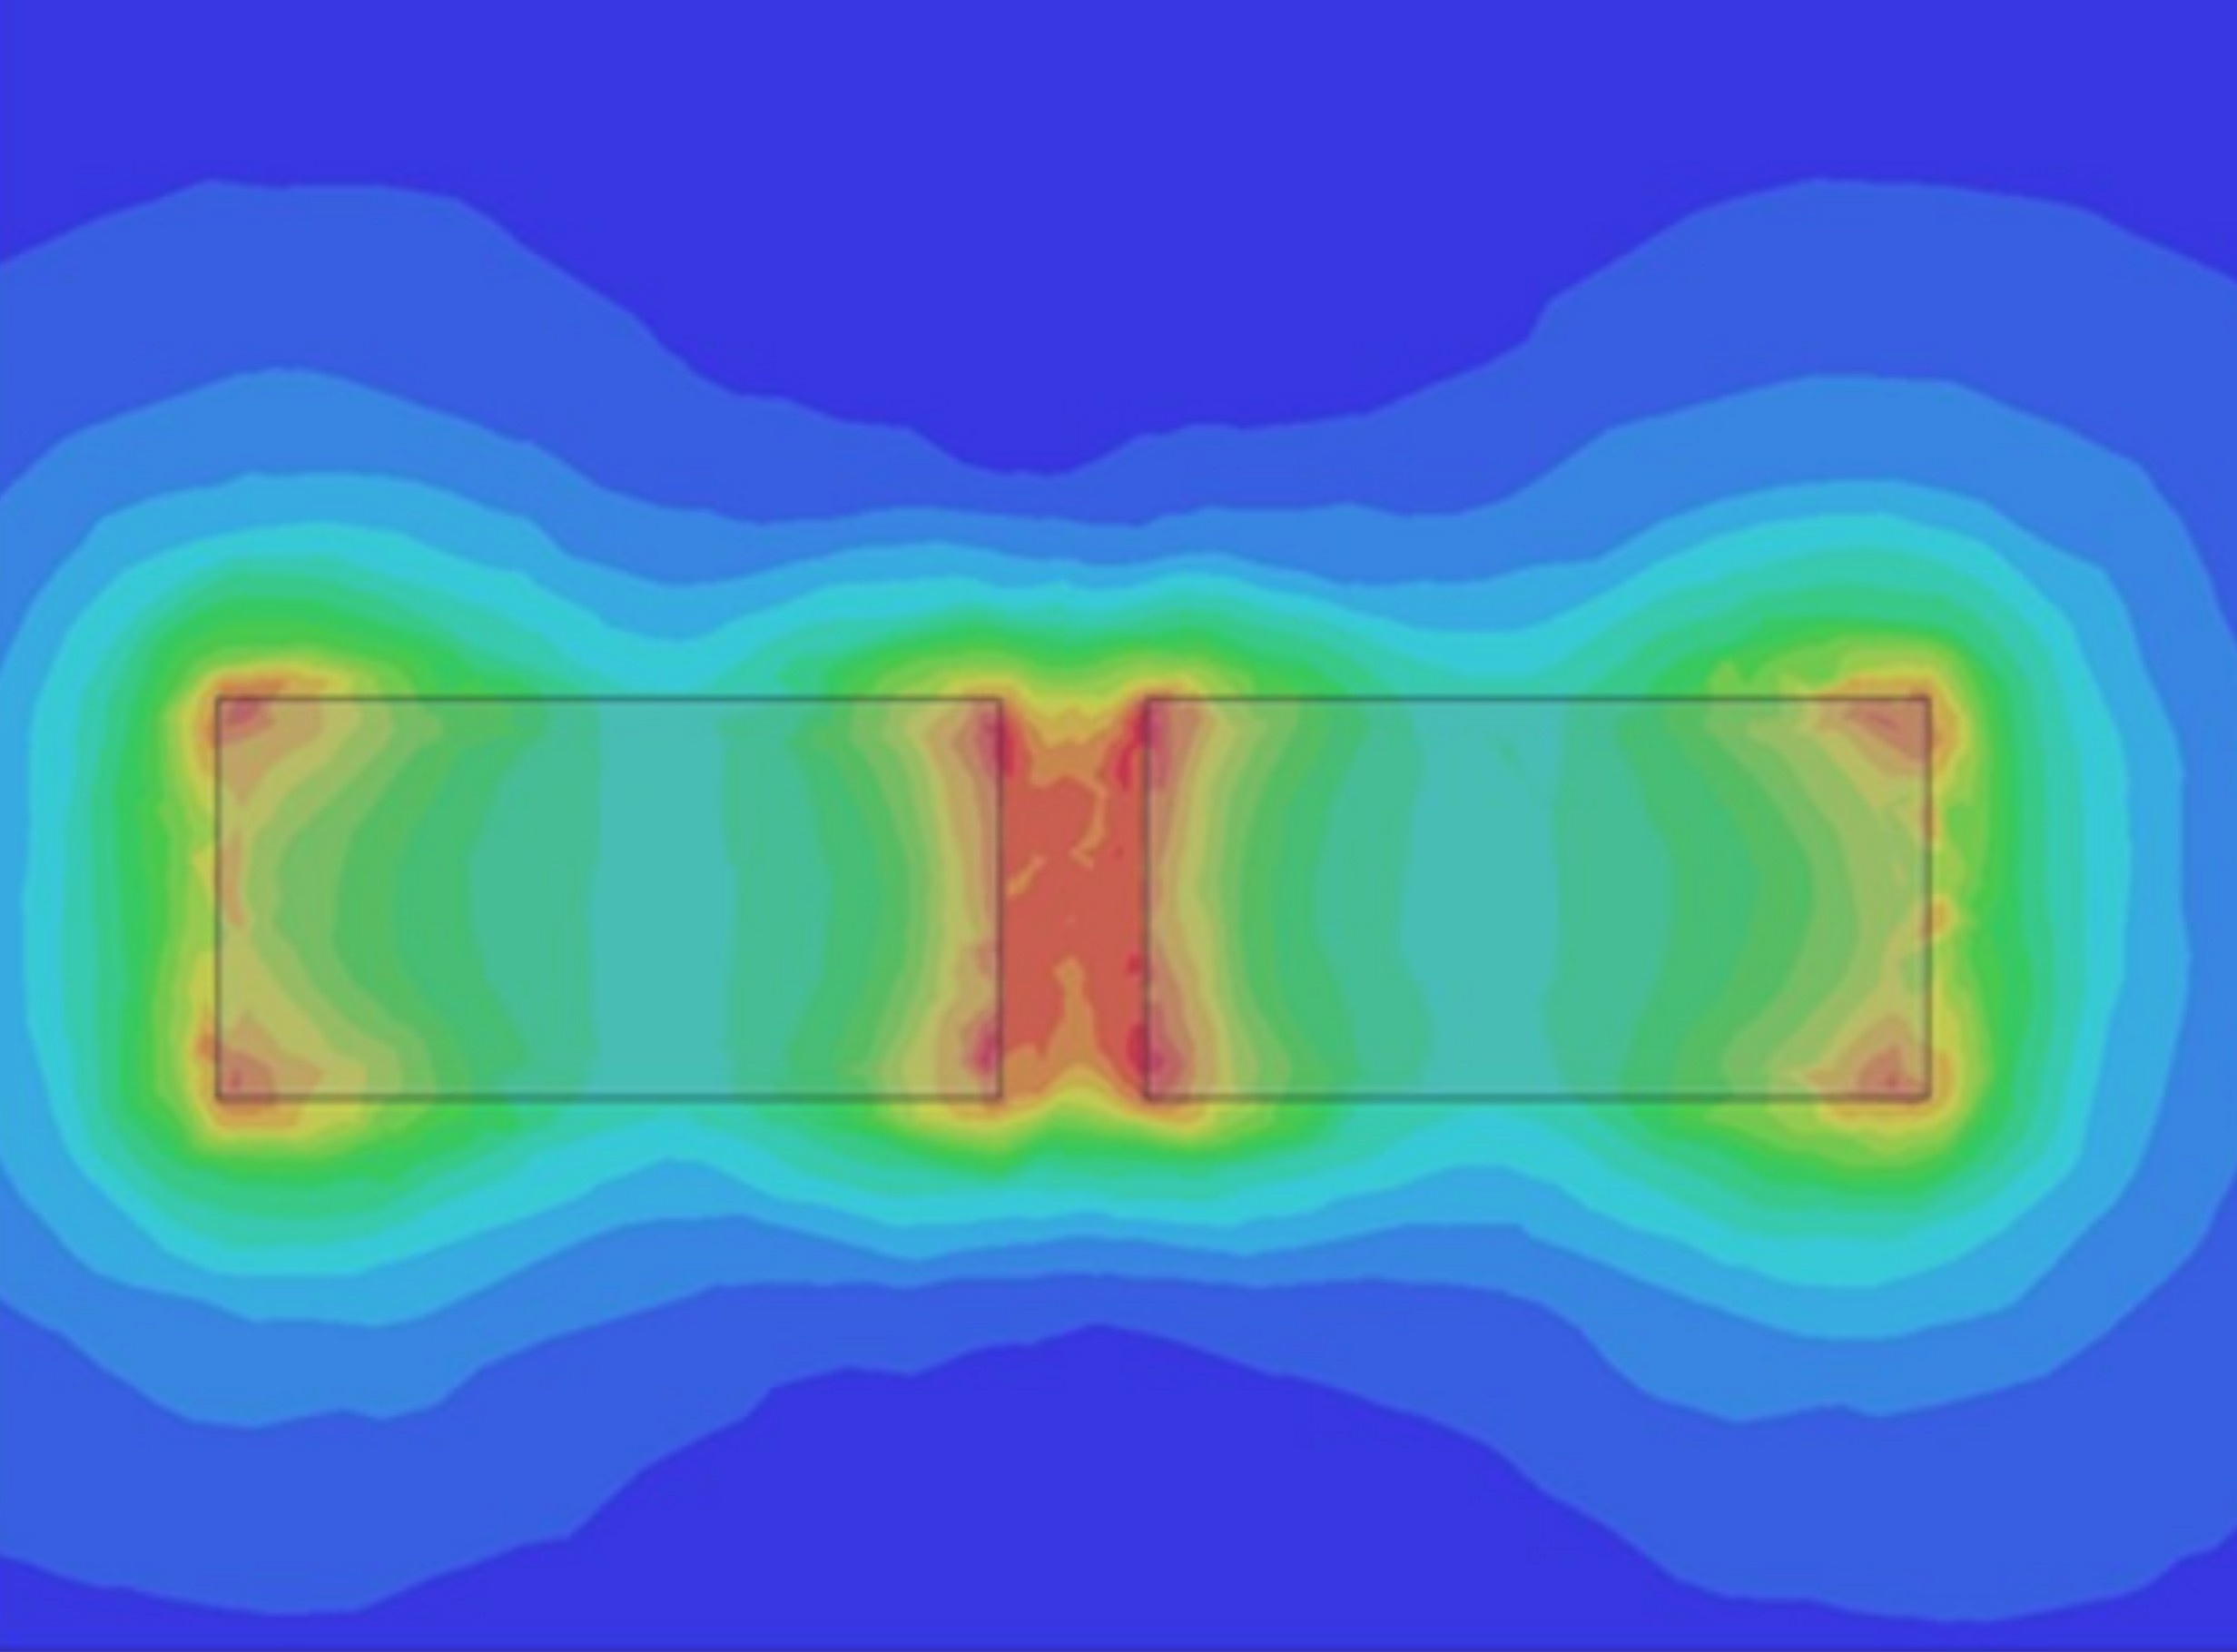
\includegraphics[height = 1.9in]{fig8_d.png}
  \label{fig:wide}} \hfil
  \caption{(a) Maximum enhancement of a gold nanodipole excited at \SI{550}{\nm} (b) narrow and (c) wide profile. A narrow structure does not maintain resonance when widened without also changing its length.}
  \label{fig:simulation}
\end{figure}
% Fig. 8 Maximum enhancement of a gold nanodipole excited at 550 nm (a) narrow and (b) wide profile. A narrow structure does not maintain resonance when widened without also changing its length.
%
when widened. However, the first resonance can be regained by changing both the length and width of the dipole as shown in Fig. \ref{fig:wide}. The mechanism causing this phenomena has to do with the manner in which surface plasmons are excited. The incident wave with a free-space wavenumber transfers energy into the plasmon wave having a much larger wavenumber at locations where the interaction between the incident wave and the antenna produce the largest concentration of higher order modes, which will couple energy into the plasmon mode. This interaction is primarily seen on the corners of the dipole in Fig. \ref{fig:wide}. Similar to plane waves in a waveguide, plasmon waves fan out from the corners taking a circuitous route bouncing from the edges of the plate before phase matching produces a resonance condition. Further complicating the picture is the chemical potential and the `lighting rod' effect whereby opposite charges form a high concentration of the field across the antenna
center gap. However, plasmons in the narrower dipole, Fig. \ref{fig:narrow}, follow a shorter, more direct route to resonance than does the plasmon wave on the wider dipole Fig. \ref{fig:wide} thereby experiencing less attenuation and ultimately creating a region of higher field enhancement in the gap than does the wide dipole. Fig. \ref{fig:sim_hi} shows that as the dipole widens the resonant frequency shifts and the enhancement decreases.  Enhancement is defined as the ratio of the total to the incident electric field in the gap region, although in some publications this ratio is squared and therefore, described as intensity enhancement.

The behavior of the narrower dipole shown in Fig. \ref{fig:narrow} is more closely aligned with what one would expect at microwave frequencies whereby increasing the length of each nanorod in plasmon half-wavelength intervals will produce successive resonance and antiresonance in the gap input impedance. Notice that the total length of the dipole is a full plasmon wavelength $\lambda_p$ plus the gap separation distance, as opposed to the typical $\lambda_0/2$ dipole first resonance of a perfectly conducting microwave antenna with a negligible gap width. In terms of plasmon wavelengths, a first resonance does occur in an isolated $\lambda_p/2$ nanorod or a vertical $\lambda_p/4$ nanorod on a metal substrate \cite{Taminiau2007}.

Although an exact determination of the plasmonic wavelength in a dielectric nanorod is not mathematically feasible, an effective wavelength $\lambda_{eff}$ based on the assumption that the antenna is a thin dielectric cylinder operating in the $\mathrm{TM}_0$ cylindrical waveguide mode has been derived in \cite{Novotny2007}. The antenna is immersed in a material with dielectric constant $\E_s$, and a Drude dielectric function is used to describe the metal rod material. The apparent increase in the antenna length at the rod ends is accounted for by an additional reactance term. This scaling law is:
%
\begin{equation}
  \lambda_{eff} = n_1 + n_2\left( \frac{\lambda}{\lambda_p} \right)
  \label{eq:lambda_eff}
\end{equation}
%
where $\lambda$ is the wavelength of the external region, $\lambda_p$ is the metal plasma wavelength, and $n_1$, $n_2$ coefficients with dimensions of length that depend on antenna geometry and static dielectric properties, are
%
\begin{subequations}
  \begin{align}
    n_1 ={}& 2\, \pi\, R \left[ 13.74 - 0.12 \frac{\E_\inf + 141.04\, \E_s}{\E_s} - 2\pi \right]
    \label{eq:n1}\\
    n_2 ={}& 0.24\, \pi\, R \frac{\sqrt{\E_\inf + 141.04 \, \E_s}}{\E_s}.
    \label{eq:n2}
  \end{align}
  \label{eq:ns}%
\end{subequations}
%
Here $R$ is the radius of the cylinder, and $\E_{\inf}$ is the dielectric constant correction in the Drude formula for $\O \gg \O_p$. For gold $\E_\inf \simeq 11$, $\lambda_p = \SI{138}{\nm}$ and for silver $\E_\inf \simeq 3.5$, $\lambda_p = \SI{135}{\nm}$ \cite{Novotny2007}.

In the case of an optical patch or dipole antenna it is necessary to account for a phase shift acquired by the surface plasmon polariton upon reflection at rod, strip, or gap terminations. The resonance wavelength $\lambda$ of metal strip resonators of thickness $t$ and width $w$ are determined approximately by \cite{Sondergaard2007}:
%
\begin{equation}
  w \frac{2 \pi}{\lambda} n_{slow} = m\pi  - \phi
  \label{eq:resonant_lambda}
\end{equation}
%
where $n_{slow}$ is the real part of the mode index of surface plasmon polaritons propagating in a metal film with the same thickness $t$ as the strip, $m = 1,2,3,\dotsc $ is the order of the resonance, and $\phi$ is the phase of the reflection coefficient at strip terminations. For a symmetric structure where $\E_d = \E_1 = \E_2$, once $t$ and $\E_m$ are selected and the phase shift $\phi$ is determined, $n_{slow}$ can be obtained from \eqref{eq:3_layer_disp} and \eqref{eq:simplified_3layer_to2layer} or for thin strips, one can use the approximation \cite{Sondergaard2008}:
%
\begin{equation}
  n_{slow} \simeq \sqrt {n_d^2 + \frac{4 \, n_d^4}{k_0^2 \, t^2 \, n_m^4}}
  \label{eq:n_approx}
\end{equation}
%
where $n_d$ and $n_m$ are the indices of refraction of the dielectric and metal and $k_0 = 2 \pi /\lambda$. The wavelength of the slow surface plasmon polariton is then given by $\lambda_{slow} = \lambda/ n_{slow}$.

Analytical models are preferable because clear trends in antenna performance can be seen by adjusting mathematical parameters that represent physical quantities such as the antenna width or length and the excitation frequency. On the other hand, numerical techniques can provide both the accuracy and flexibility needed to model complex antenna structures. However, purely mathematical solutions can become clouded with long complex expressions and special functions while a purely numerical analysis provided by the powerful commercial codes that have become available these last few years, while furnishing useful visual data in terms of graphs and charts, do not always provide a way to understand the multifaceted interaction between the variables of an antenna system. Recently a compromise approach for optical antennas has been advanced, advocated primarily by Engheta and Alù \cite{Engheta2005,Alu2007,Zhao2011,9781107014145}, whereby the antenna and field excitation are replaced by an equivalent lumped circuit model based on
numerical analysis data. The basic model, shown in Fig. \ref{fig:alu_circuit}, is centered on a Thévenin equivalent circuit for the antenna with a capacitance accounting for a non-negligible gap
impedance $Z_g$ along with the intrinsic impedance $Z_a$ of the dipole. The parallel combination of these two impedances forms the input impedance of the circuit. The input impedance is calculated, by driving the antenna at the gap with an arbitrary source voltage $V_g$ and calculating, with full-wave simulations, the displacement current $I_g$ flowing across the arms at the terminals in the region of the gap $Z_{in} = V_g / I_g$.

The intrinsic antenna impedance $Z_a$ is extracted from the input impedance by first taking the parallel combination of the gap and load impedances according to:
%
\begin{equation}
  Z_{in} = \frac{1}{1 / Z_a + 1 / Z_g}, \quad  Z_g = \frac{1}{\j \O \,C}, \quad \text{where} \,C = \E_0 S/g
  \label{eq:alu_impedance}
\end{equation}
%
where $S$ and $g$ are respectively the gap cross-sectional area and gap height. Setting $Z_a = R_a + \j X_a$ and $Z_{in} = R_0 + \j X_0$,  \eqref{eq:alu_impedance} is rearranged to give:
%
\begin{subequations}
  \begin{align}
    R_a ={}& \frac{R_0}{1 + \O \, C \,\left( 2 X_0 + \O \,C \,(R_0^2 + X_0^2) \right)}
    \label{eq:intrinsic_resistance}\\
    X_a ={}& \frac{X_0 + \O \, C \,(R_0^2 + X_0^2)} {1 + \O \, C \,\left( 2 X_0 + \O \, C \,(R_0^2 + X_0^2) \right)}.
    \label{eq:intrinsic_admittance}
  \end{align}
  \label{eq:instrincis_impedance}%
\end{subequations}
%
Since full-wave simulations have provided the $Z_{in}$ components $R_0$ and $X_0$, the dipole intrinsic impedance is determined mathematically from \eqref{eq:instrincis_impedance}. The intrinsic impedance $Z_a$, which is unaffected by antenna loading either by a transmission line or by altering the gap capacitance, is now completely determined.

The antenna is resonant when the input reactance $X_0 = 0$ which from \eqref{eq:intrinsic_admittance} is:
%
\begin{equation}
  \O_{0} = \frac{X_a}{C  (R_a^2 + X_a^2)}
  \label{eq:resonant_frequency_impedance}
\end{equation}
%
The `open circuit' or first resonance has been shown to have a very low value, whereas the `short circuit' or antiresonance has a high impedance, on the order of kilo-ohms. The feed line or other loading conditions will determine which operating frequency is selected. In the event of loading, the capacitance becomes $C = \E_L S /g$, the new resistance and reactance terms in the input impedance $Z_{in} = R_{in} + \j X_{in}$ are again found numerically and the equivalent dielectric constant $\E_L$ can be calculated from \eqref{eq:intrinsic_admittance}. Extra circuit elements can be added to account for the transmission feed line or a quantum radiator such as is the case in molecular spectroscopy, or a different circuit can be created for single quantum radiators without a gap \cite{9781107014145}.
%
\begin{figure}[b!]
  \centering
  \def\svgwidth{.75\linewidth}
  \input{figures/alu_impedance.pdf_tex}
  \caption{Optical antenna with equivalent circuit model. The driving voltage could be an incident electromagnetic field, a transmission line connected to the antenna, or a quantum emitter.}
  \label{fig:alu_circuit}
\end{figure}
%
% Fig. 9 Optical antenna with equivalent circuit model. The driving voltage could be an incident electromagnetic field, a transmission line connected to the antenna, or a quantum emitter.
Efficiency is an important measure used to characterize antenna performance. The overall antenna efficiency can be broken down into the product of several measures of efficiency, the most important of which are the radiation efficiency and the reflection efficiency, $\eta  = \eta_{rad}\eta_{ref}$,
where the maximum value of each efficiency is one. The reflection efficiency determines how well the transmission feed line characteristic impedance is matched to the antenna input impedance. Its value, given in terms of the transmission line reflection coefficient $\Gamma$, is $\eta_{ref} = 1 - \left| \Gamma  \right|^2$ where $\left| \Gamma \right| \le 1$. The radiation efficiency is ratio of the total power radiated $P_{rad}$ to the power received $P_{in}$ by the antenna. The input power is assumed to be the sum of the radiated power and the power losses on the antenna. Provided the antenna is fed at the antenna maximum current point, which is most often the case with optical antennas operating at or below the lowest resonant frequency. At the first antiresonance, the radiation efficiency can be expressed in terms the radiation resistance $R_{rad}$ and the ohmic loss resistance $R_L$ experienced by the current flow in the antenna elements. The radiation efficiency is therefore:
%
\begin{equation}
  \eta_{rad} = \frac{R_{rad}}{R_{rad} + R_{in} \sin^2(\pi \, L_{eff}/{\lambda _{eff})}}; \quad  R_{rad} = 2 P_{rad}/I_{max}^2.
  \label{eq:rad_efficiency}
\end{equation}
%
The ohmic loss resistance $R_{in}$ is the real part of the input impedance. The optical dipole radiation resistance can be determined analytically by first hypothesizing the current at resonance. Taking into account the effective length and wavelength of an optical antenna, $L_{eff}$ and $\lambda_{eff}$  respectively which can be calculated using \eqref{eq:lambda_eff}, the standard microwave expression for a dipole current is modified to become \cite{Alu2007},
%
\begin{equation}
  I(z) = \ddfrac{I_0 \sin \left [\pi \frac{L_{eff} - 2|z|}{\lambda _{eff}}\right]} {\sin \left( \frac {\pi \, L_{eff}}{\lambda_{eff}} \right)}
  \label{eq:current}
\end{equation}
%
where $I_0$ is the numerical displacement current at the feed point $z = 0$. This current \eqref{eq:current} is used to find an analytical expression for the power radiated by the optical dipole $P_{rad}$ which is then substituted into \eqref{eq:rad_efficiency} to find the efficiency.

Antenna directivity defined as $D_0$ = (time average power density maximized with angle)/(average total power radiated through a sphere), can again be analytically calculated with the formulas above as can gain which is the product of the efficiency times the directivity, $G_0 = \eta_{rad} D_0$ . Keep in mind that this exercise has been a combination of numerical and analytical calculations, forming a hybrid approach that seems best suited for understanding complex interactions as well as for overall engineering optical antenna design.  Although the example of a dipole has been used here, many other structures have been successfully investigated using this equivalent technique \cite{Zhao2011,9781107014145}. For design data for the dipole based on measurements the reader is referred to references \cite{Schuck2005,Fischer2008,Muskens2007}.
%%
%%
%%
\subsection{Bowtie Antenna}
%
Compared to a dipole antenna, the bowtie antenna has the advantage of broadband operation yet it is a simple design. The feed point of a bowtie antenna is a gap at the vertex of two tip to tip apposal triangular electrically conducting arms. If extended to infinity while the angles of the triangle vertices remain unchanged, this antenna would be frequency independent. When the incident field polarization is perpendicular to the gap, the antenna can be driven into resonance. Fig. \ref{fig:s_bowtie} shows the intensity distribution for a \SI{520}{\nm} resonant bowtie design made out of gold on a $\text{SiO}_2$ substrate and excited by a normally incident plane wave. The numerical simulation in Fig. \ref{fig:s_bowtie_1} shows that a high field intensity distribution occurs not only at corners and in the gap region but also along each of the sides, likely due to the sharp edge design. In Fig. \ref{fig:s_bowtie_2} a plot of the electric field vectors immediately above the surface of antenna indicate the largest field components are just above the gap region but tend to decrease in amplitude as they spread out and terminate at the wider ends of the antenna arms where a much lower intensity is seen in Fig.
\ref{fig:s_bowtie_1}. The intensity of the field in the bowtie gap has been shown
to be strongly dependent upon the gap width \cite{Schuck2005}. For the design presented in \cite{Schuck2005}, starting on the order of \SI{50}{\nm} the resonant intensity climbs exponentially as the gap separation narrows, however as the gap separation widens the intensity tends to level out at around \SI{100}{\nm}. Although very little work has been carried out concerning mathematical design criteria for the construction of on-surface optical antennas, optimal design dimensions can be obtained through published data gathered in experiments. For optical frequency design data based on measurements for the bowtie antenna the reader is referred to reference \cite{Fischer2008}. Studies have also been carried out to determine optimum bow angle, the outside angle formed by the edges of the two apposal arms of a bowtie antenna. It has been reported that the strongest enhancement can be obtained with a bow angle of \SI{90}{\degree} \cite{Fischer2008}.
%
\begin{figure}[t!]
  \centering
  \subfloat[]{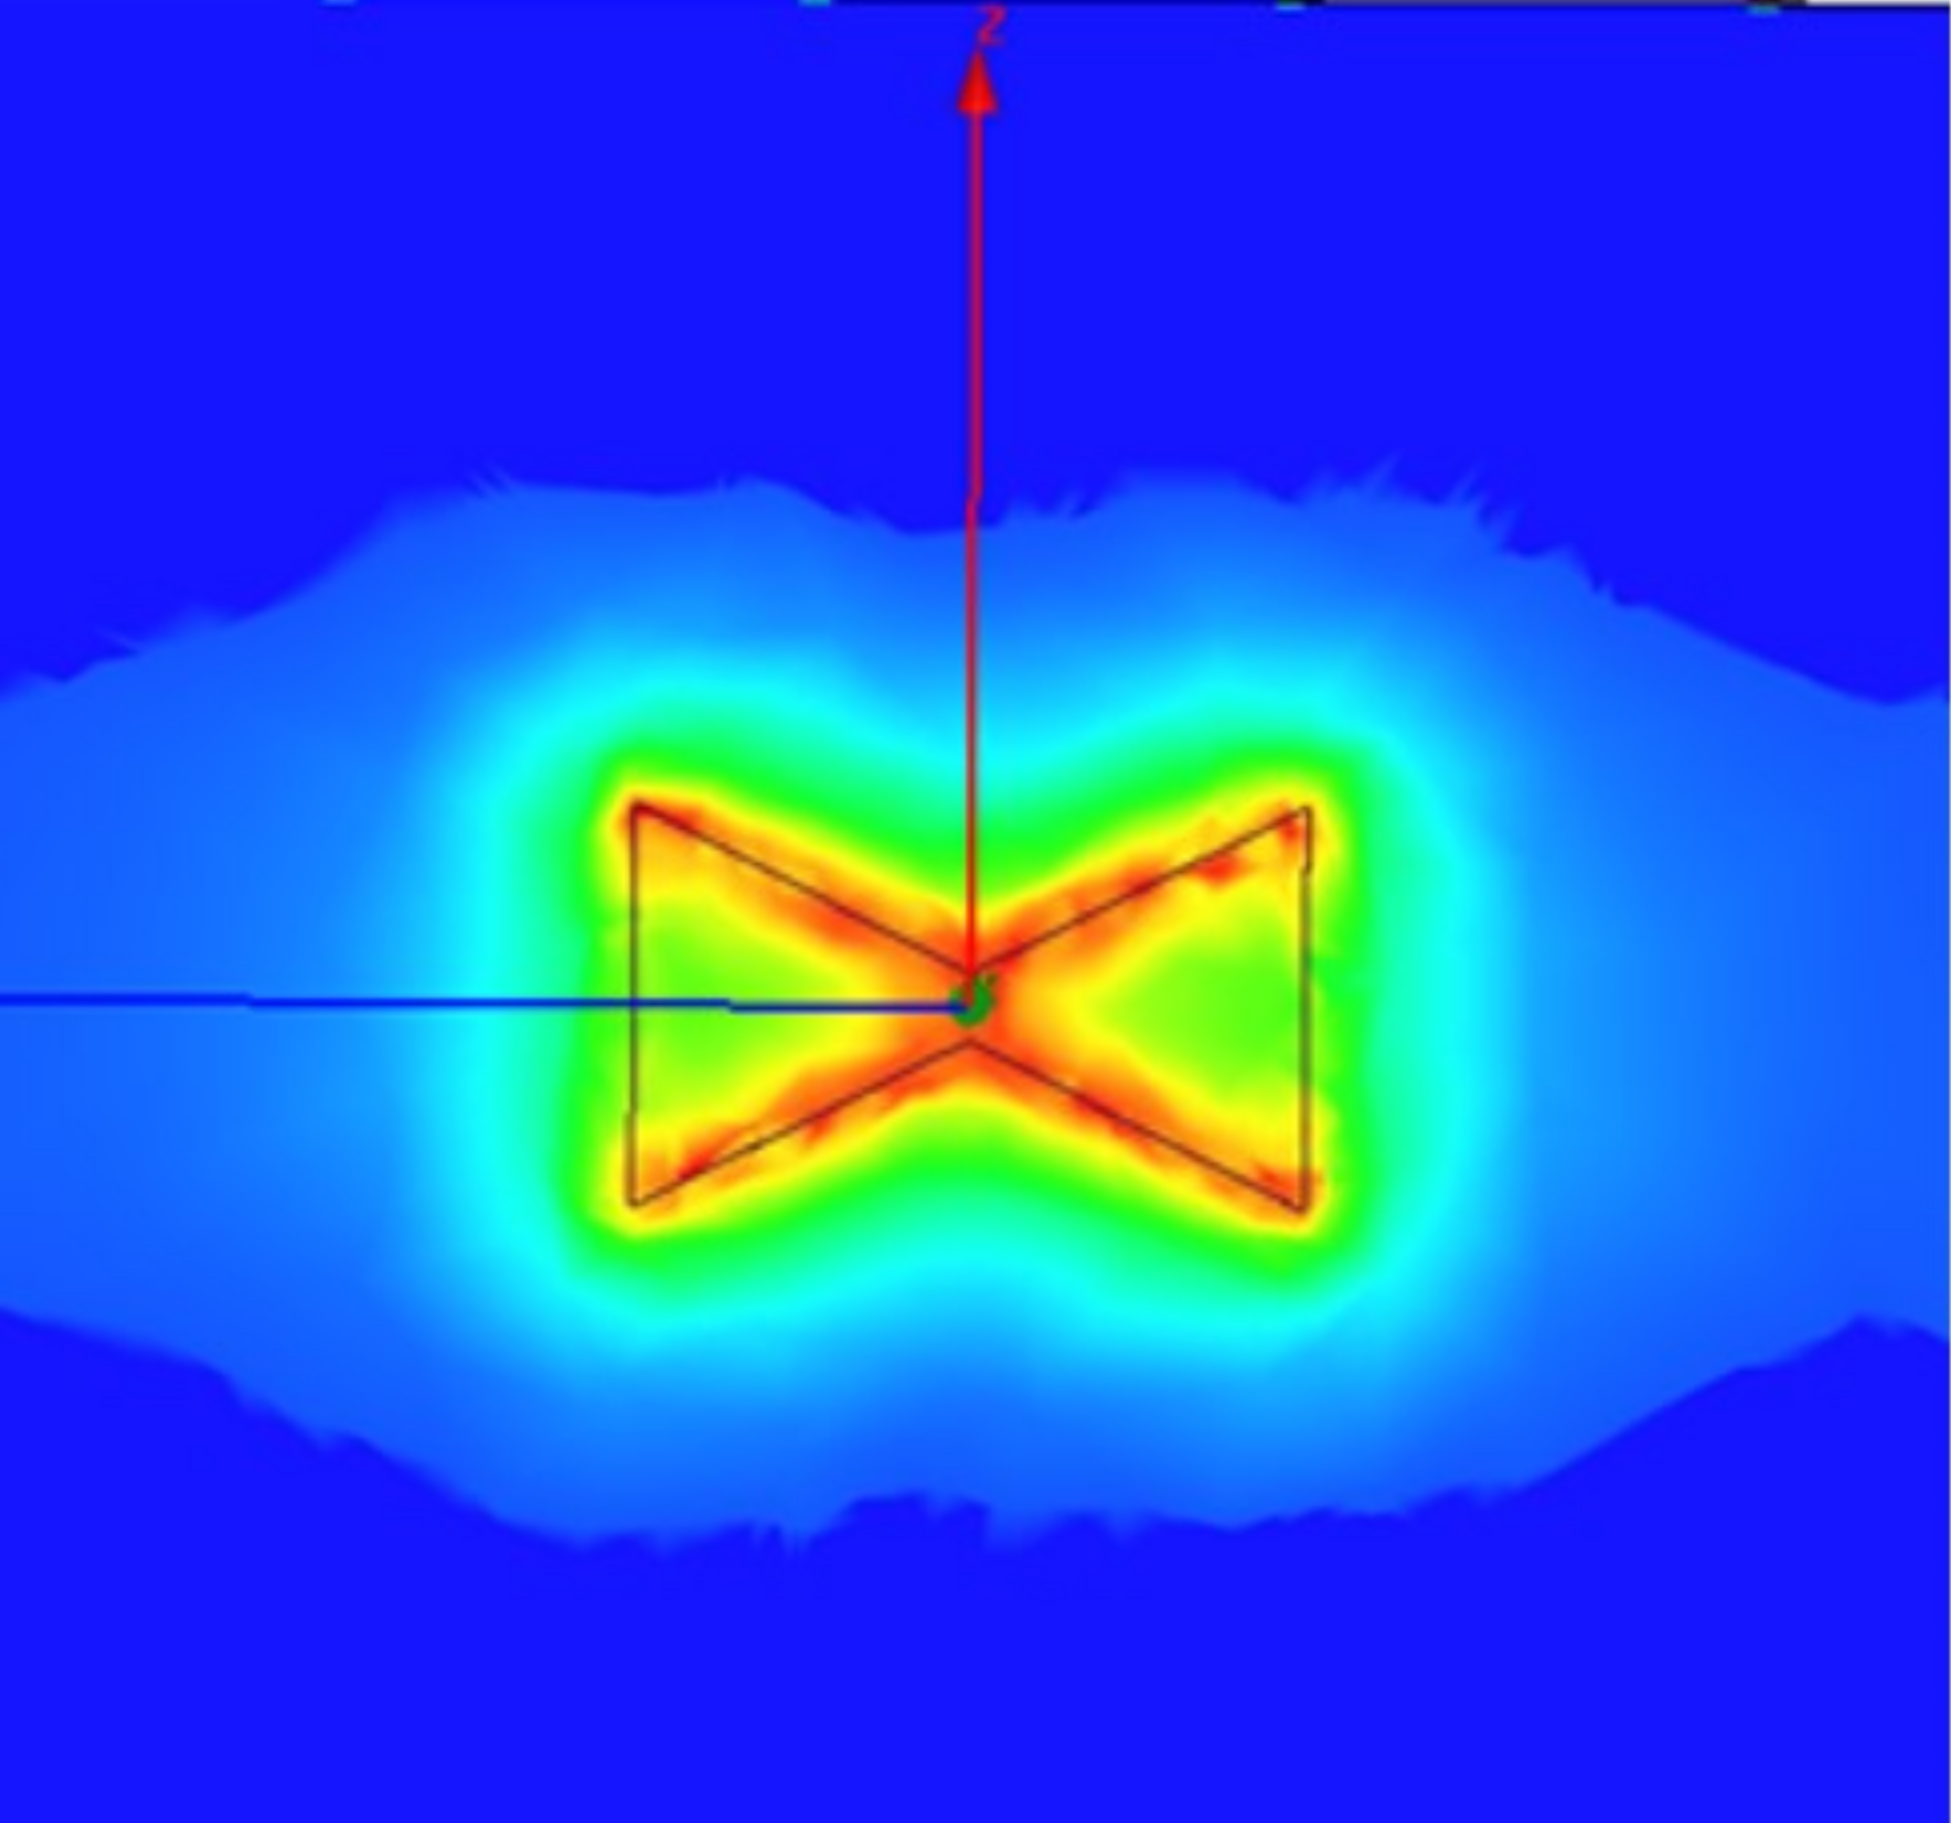
\includegraphics[height = 1.9in]{fig10_a.png}
  \label{fig:s_bowtie_1}} \hfil
  \subfloat[]{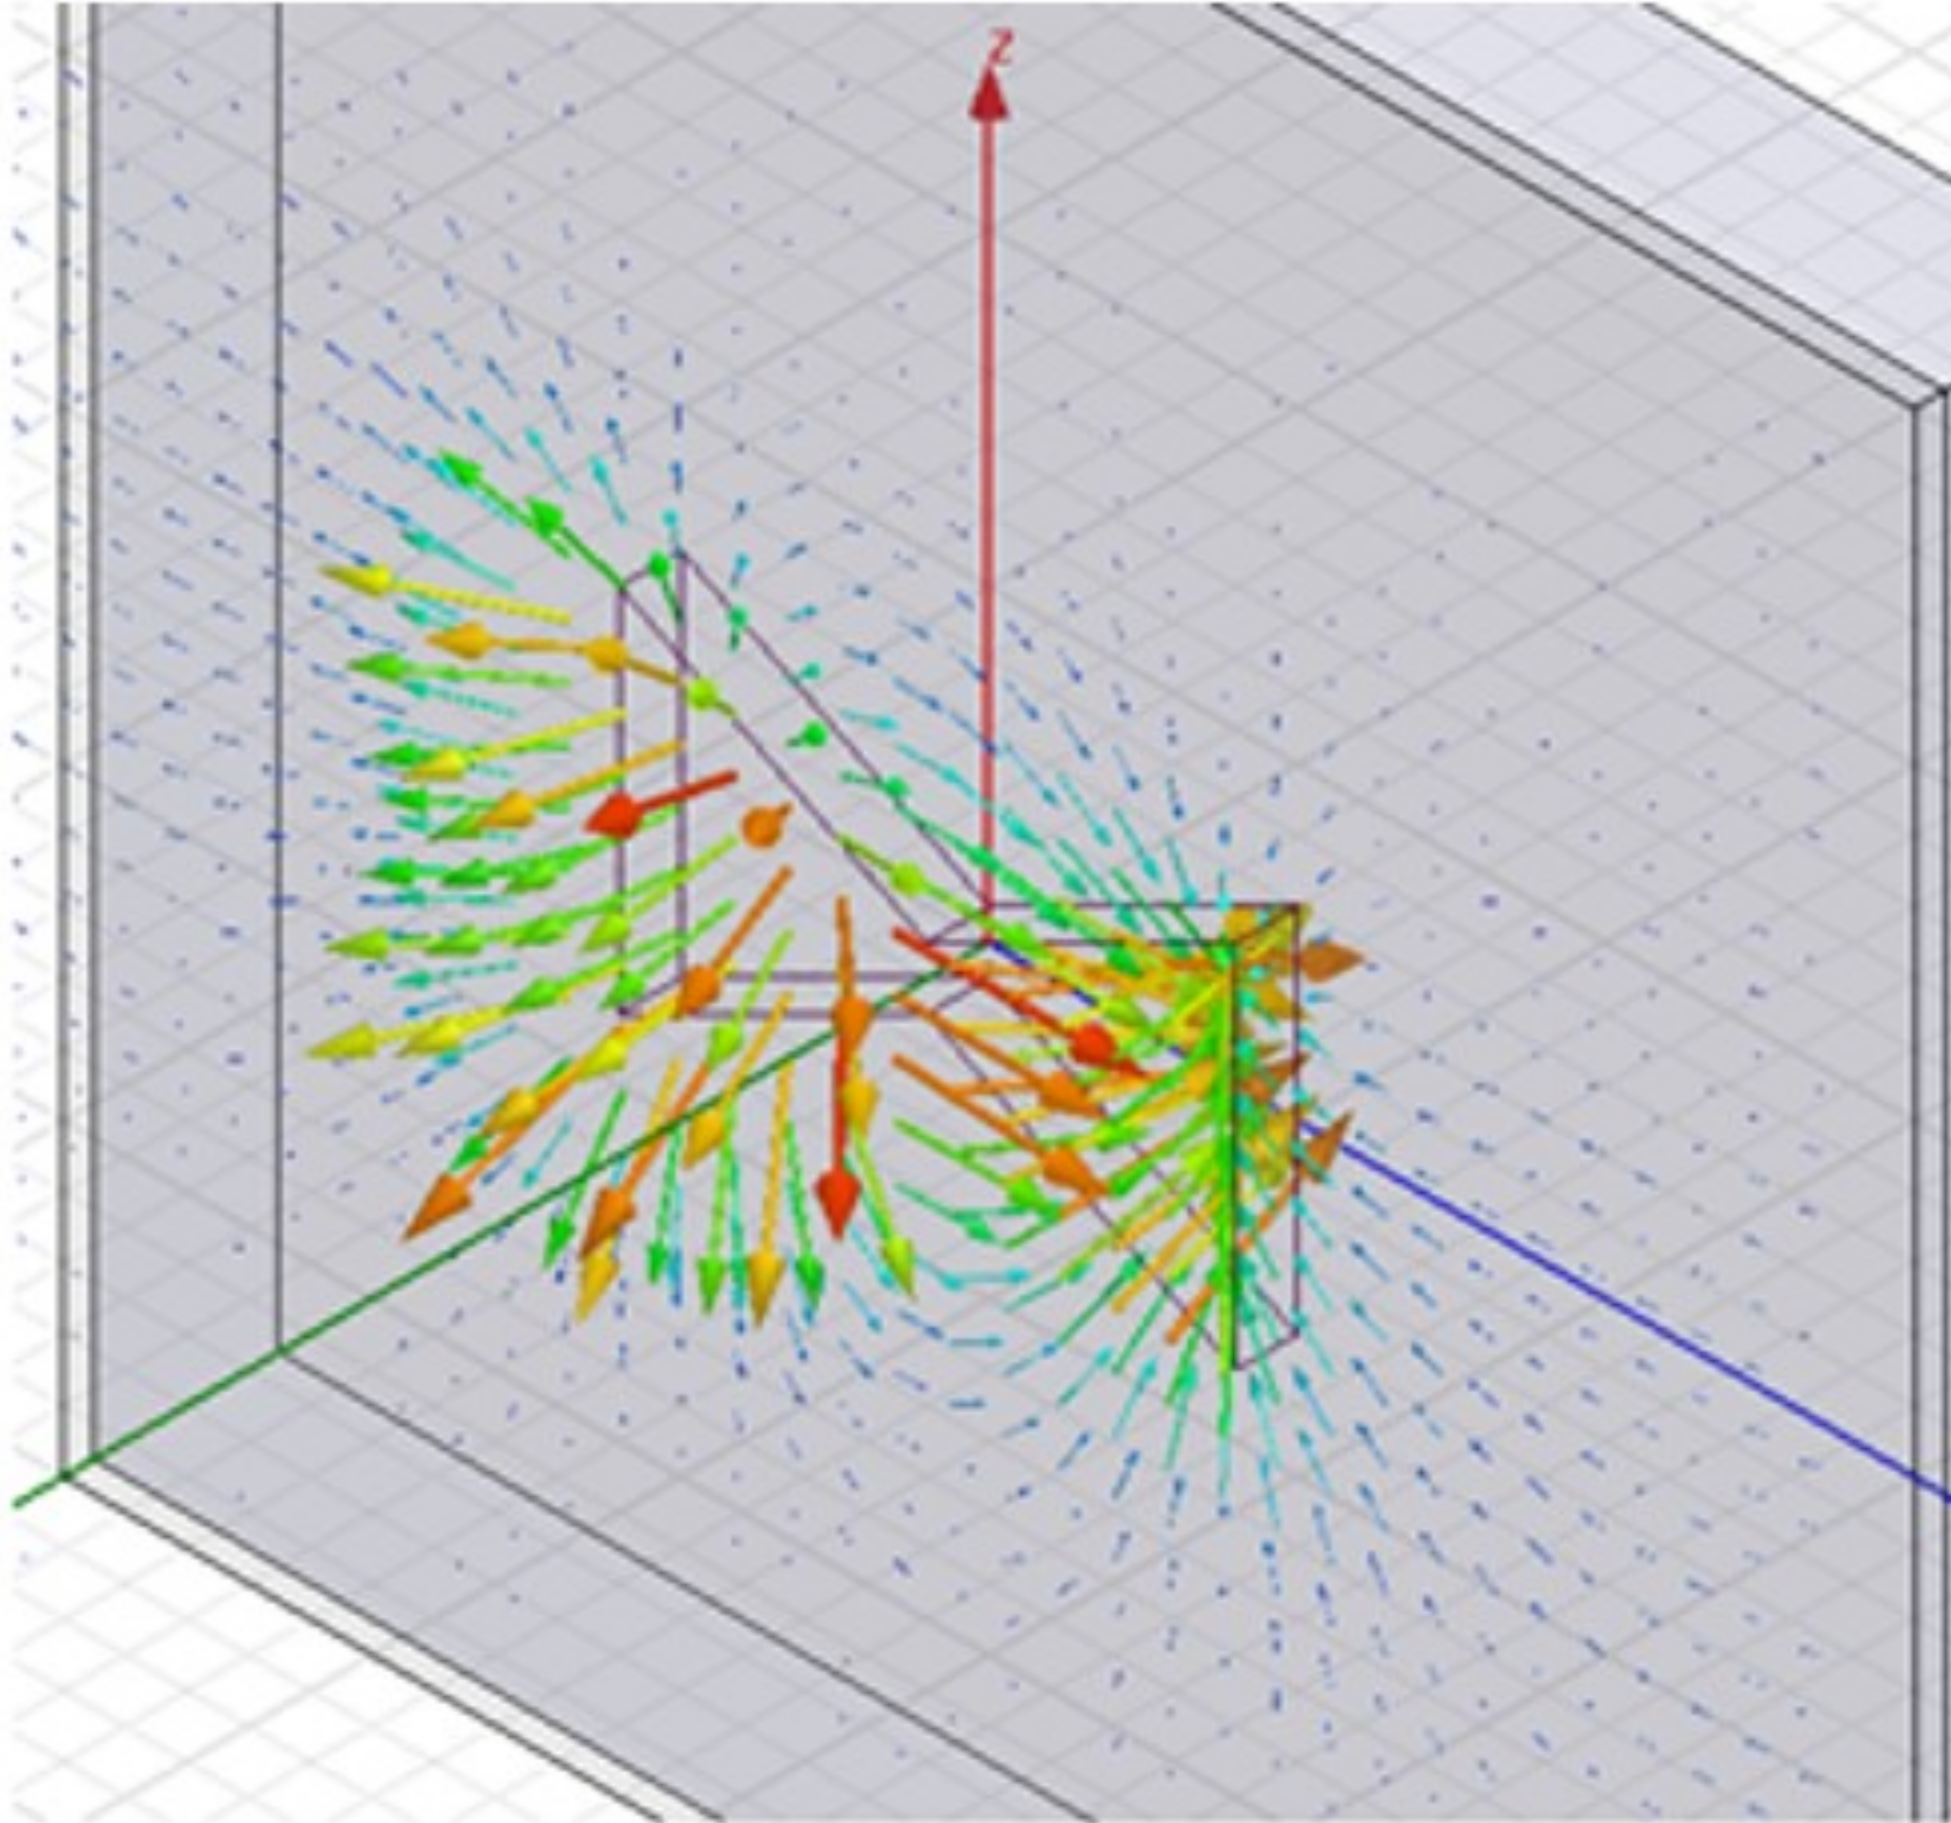
\includegraphics[height = 1.9in]{fig10_b.png}
  \label{fig:s_bowtie_2}} \hfil
  \caption{Bowtie antenna with (a) highest field intensity shown in red around the edges and corners of the triangular arms and (b) electric field vectors where the largest amplitude field is displayed in red occurs in the gap between the two arms.}
  \label{fig:s_bowtie}
\end{figure}
% Fig. 10 Bowtie antenna with (a) highest field intensity shown in red around the edges and corners of the triangular arms and (b) electric field vectors where the largest amplitude field is displayed in red occurs in the gap between the two arms.
%
Unlike microstrip antennas printed on a thin substrate with a metal backing focusing radiation into the air region above, optical antennas are a single metal radiator lying on a dielectric-air interface. There can be no ground plane below because there are no perfect conductors at optical frequencies. Although radiation is in both directions, most of the energy radiated from an optical antenna tends to couple into the higher density substrate. In the microwave case a $\text{TM}_0$ mode surface wave can be launched into the substrate because this mode has no cutoff wavelength, but the fundamental mode in a typical microwave patch antenna is not conducive to launching TM modes. As long as the substrate is thin, a microwave patch antenna suffers little substrate induced loss. As the substrate thickens, energy from the microwave patch antenna is coupled into surface wave modes, which seriously degrades the efficiency of an antenna. However, an optical antenna radiates in both directions regardless of the substrate thickness, making it in any case less efficient than its microwave counterpart. One measurement study carried out in
the infrared range \cite{Fischer2008} concluded that the dipole and bowtie efficiencies are respectively \SI{20}{\percent} and \SI{30}{\percent} whereas a typical microstrip patch antenna has an efficiency of \SI{60}{\percent}. A similar conclusion was reached in a more recent study \cite{9781107014145} that included the optical dipole, bowtie, and dimer constructions. A dimer, which has two pancake shaped arms, has an efficiency level close to the bowtie design. Numerical investigations of the optical Yagi-Uda design show a strong emission into the substrate and a much smaller emission lobe into the air side of the surface \cite{Hofmann2007} \cite{Kosako2010}. Although most of the electromagnetic radiation is emitted into the critical angle below, the above surface emission still shows a strong directivity.
%%
%%
%%
\subsection{Yagi-Uda Antenna}
%
The dipole and bowtie nanoantennas described above are most often used in applications where a wide beamwidth or broadband transmission is the primary objective. However as nanotechnology progresses, achieving highly directional beams in the optical regime will be necessary in order to, for instance, transmit signals from nanocircuits to a receiver above the surface with a minimum power load on the electronic system. Another significant application is the possibility of enhancing and directing the radiation from a nano-emitter, which will be discussed in the \emph{Applications} section below. At the microwave level the Yagi-Uda antenna shown in Fig. \ref{fig:yagi_uda} has proven to be highly directional for radiation of radio waves yet simplistic in construction. One would expect that basically similar design principles can be used to obtain directionality with an optical Yagi-Uda design. Over the last few years, this has been shown to be the case primarily due to the fact that the elements of the Yagi antenna are nanorods, the properties of which have been the subject of extensive study by the optics community over the last thirty years.
%
%
\begin{figure}[h!]
  \centering
  \def\svgwidth{.75\linewidth}
  \input{figures/yagi.pdf_tex}
  \caption{Yagi-Uda optical antenna constructed with nanorods.}
  \label{fig:yagi_uda}
\end{figure}
% Fig. 11 Yagi-Uda optical antenna constructed with nano rods.
%
%
The essential Yagi-Uda design consists of a resonant driven element flanked on one side by a longer passive reflector element and on the other by a series of shorter director elements, all of which lie in the same plane. Researchers have studied a variety of element types for the Yagi, including spheres and prolate spheroids, but low efficiency and difficulties in achieving smooth surfaces and precise positioning on the nano level has focused attention on the classical cylindrical rod design. In addition to surface smoothness and the precise rod length and positioning needed for optimum array performance, other difficulties encountered in the optical regime are the loss of energy coupled into the substrate, the difference in wavelength between free-space and the metallic rods, and field interaction with the air-substrate boundary causing a phase difference between surface plasmons on the two sides of the antenna. Naturally these effects can be modeled by pure numerical calculations but preventing unwanted consequences such as the substrate energy loss are still left open for future research. However detailed design rules have been developed
\cite{Hofmann2007} for the optical Yagi. As a rough estimate high directivity can be obtained with separation distances of about $0.25\, \lambda$ between the feed and the reflector and about $0.3\, \lambda$ between the feed and the director and between each of the director elements \cite{Kosako2010}. The length of the feed element is the effective resonant wavelength $\lambda_{eff}$ of the antenna rods which is related to the incident free-space wavelength $\lambda$ by a simple relation given in \eqref{eq:lambda_eff} above with an accompanying discussion.

A scanning near-field optical microscope (SNOM) has been used to simultaneously image the amplitude and phase of the normal electric field component on a working Yagi-Uda nanoantenna \cite{Dorfmuller2011}. This data was processed to produce a time evolution animation of the fields of the antenna during reception, providing an unusual opportunity to check time domain numerical simulations of the received fields. These measurements showed that illumination of the antenna from the forward direction resulted in constructive interference of scattered light by the antenna elements which leads to a strong field enhancement in the feed element. Measurement data taken when illumination is from the rear of the antenna reveal that the destructive interference by the feed element suppresses strong fields.
%%
%%
%%
\subsection{Log-Periodic Antenna}
%
To date, most theoretical and experimental studies on directional optical antennas have focused on the Yagi-Uda design, shown in Fig. \ref{fig:yagi_uda}, which provides good directivity for a specific design frequency with a limited bandwidth. A possibility of improving both bandwidth and directivity may be met with a log-periodic antenna design. The name is derived from a progressive spacing between the elements of the antenna based on a logarithmic scale. A number of log-periodic design schemes have been employed at microwave frequencies. At optical frequencies several graded size and spacing designs have been proposed with elements varying in shape from spheres and ellipses to the classical elongated rod. Due to difficulties in creating precise size and shapes at the nano level most implementations are only approximations of the true log-periodic requirement.

In a log-periodic antenna arrangement \cite{Balanis2015}, the arm lengths $l_n$, spacing between arms $R_n$ and rod diameters $d_n$, increase logarithmically as defined by the inverse of the geometric ratio $\tau$ as given by:
%
\begin{equation}
  \frac{1}{\tau} = \frac{l_{n + 1}}{l_n} = \frac{R_{n + 1}}{R_n} = \frac{d_n}{d_{n + 1}}.
  \label{eq:logperiodic}
\end{equation}

Another parameter associated with the array, but independent of the geometric ratio, is the scaling factor. The scaling factor is often expressed normalized by the element length and as such it is given by $\sigma  = d_n/ {2 l_n}$. The half angle at the antenna apex is determined by the parameters $\tau$ and $\sigma$ according to $\A  = \tan ^{-1}\left[(1 - \tau)/{4 \sigma} \right]$.

In one study \cite{Pavlov2012}, measurements were carried out on an optical log-periodic antenna with gold elements on a glass substrate strictly following the design criteria above. However unlike other optical array designs, a gap was placed in the middle of each arm in order to enhance the field produced by plasmonic action. It was observed that the directionality of the antenna reaches a maximum with $N = 10$ elements but the optimum field enhancement value of $|E_{FB}|^2$ for the forward beam electric field is obtained between $N = 6$ and $N = 10$. A decrease of the field enhancement values, defined as $|E_{total}|^2/|E_{inc}|^2$ with increasing numbers of elements is associated with increasing plasmonic losses incurred in the addition of elements. Adding a gap did not affect the antenna patterns, however a significant increase in beam intensity was observed. As with other on-surface plasmonic antennas, a significant portion of the radiated power is coupled into the substrate.

One of the drawbacks of the log-periodic design is that the currents in the optical version have the same phase in each element. In addition, the elements are closely spaced producing a phase progression of the current in the direction of the longer elements. This produces an end-fire beam in the direction of the longer elements and interference effects in the pattern. The standard design for a log-periodic antenna calls for crisscrossing the feed between adjacent elements thereby adding a $180\degree$ phase shift to the terminal of each element. Since the shorter elements are spaced closer together and opposite in phase, very little energy is radiated from them and interference effects are minimal. The radiation pattern in this crisscross case tends to be toward the shorter elements \cite{Balanis2015}. In the previous paragraph, the design calling for dipoles rather than solid rods appears to be a step in the right direction. The plasmonics of optical frequency materials and construction methods on the nano level will determine the efficacy of adapting the standard microwave design where alternate dipoles are connected.
%%
%%
%%
\subsection{Purcell factor}
%
Light emission from an optical quantum emitter such as a quantum dot or a nano-crystal can be enhanced when it is in close proximity to an intense electromagnetic source. This effect was first discovered at radio frequency by E. M. Purcell, when he observed an increase in the probability of spontaneous emission of an emitter placed in a resonator \cite{Purcell1946}. However, controlling the degree of enhancement of a quantum emitter remains a major challenge. Optical microcavities or microresonators such as optical nanoantennas, generally used for emission enhancement can be mathematically quantified by what has become known as the Purcell factor $F$ \cite{Vahala2003}, defined as:
%
\begin{equation}
  F = \frac{3}{4 \pi^2} \frac{ \lambda}{n} \times \frac{Q}{V}
  \label{eq:purcell}
\end{equation}
%
where $\lambda$ is the wavelength of the emitted photon, $Q$ and $V$ are the quality factor and mode volume respectively, and $n$ is the refractive index of the surrounding medium. The $Q$ corresponds to the temporal confinement while the mode volume $V$ represents the spatial confinement. Although cavity based structures can provide very high $Q (\sim 10^4)$ \cite{Song2005}, they are consequently narrow bandwidth devices. This spectral limitation is a problem for contemporary solid-state quantum emitters which, despite many efforts in research, still have a broad spectral emission due to stability issues \cite{Gaebel2004}.

Optical nanoantennas, on the other hand have a much lower $Q (\sim 100)$ \cite{curtothesis} and hence are suitable for applications involving broadband sources. However, due to surface plasmon polaritons, they have the capability to highly confine the light source volume well beyond the diffraction limit \cite{Maier2006,Barthes2011}. Coupling optical nanoantennas with quantum structures like quantum dots can result in highly directive quantum emitter intensity pattern, but with a mode volume as low as $.002 \left(\lambda/n \right)^3$ \cite{curtothesis} which corresponds to a very high Purcell factor of $\sim \SI{5e4}{}$.
%%
%%
%%
\subsection{Aperture Antennas}
%
So far in this chapter on-surface optical antennas have been emphasized primarily because there is considerable current scientific and industrial interest in the design of antennas for optical and near infrared communications. However, there is also significant industrial interest in antennas that are effective in focusing light to sub-wavelength dimensions. A primary application lies in the possibility of extending current photolithographic techniques to produce circuit chips on a sub-wavelength scale using relatively inexpensive optical equipment as compared to ion-beam etching machines. Nano-aperture antennas have been the key component in sub-wavelength lithographic research and also been a key element in the development of several other technologies that will be discussed in the \emph{Applications} section. Below a brief treatment of the theory of optical aperture antennas is presented followed by an overview of selected designs that have received popular attention in the literature.
%%
%%
%%
\subsection{Optical aperture antenna theory}
%
Although important nano-level aperture optics was carried out in the study of fluorescence molecules in the 1980's \cite{Fischer1986}, the report by \cite{Ebbesen1998} of dramatically enhanced transmission through sub-wavelength holes in metal films, was an event that spurred widespread interest in optical aperture antennas. Because this phenomena, now known as extraordinary optical transmission (EOT), seemed to fly in the face of the widely accepted classical electromagnetic analysis by \cite{Bethe1944} and \cite{Bouwkamp1950}, there has been considerable scientific interest in the subject reaching to the core of surface plasmon theory. According to the classical theory, the power transmitted through an aperture in an infinitely thin metallic screen scales as the inverse fourth power of the aperture size in terms of wavelengths. If the screen is made to be of finite thickness, then an additional reduction in the transmitted field strength will result, due the below-cutoff dimensions of the slot. However, it was discovered, first experimentally and then confirmed by
numerical analysis, as shown in Fig. \ref{fig:cst_simulation}, that for metals at optical frequencies there are situations where remarkable
%
\begin{figure}[h!]
  \centering
  \subfloat[]{\includegraphics[width = .75\linewidth]{fig_13.png}}
  \caption{Simulation showing a surface plasmon standing wave intensity ($|E|^2$) pattern on a thin silver plate with dielectric constant $\E= -18.242 + \j 1.195$ between two slots illuminated by a \SI{660}{\nm} plane wave from below. The center plate has a length $5/2 \lambda_{spp}$ (\SI{1650}{\nm}) and each aperture has a width and thickness of \SI{200}{\nm}.}
  \label{fig:cst_simulation}
\end{figure}
% Fig. 13 Numerical calculation (CST©) showing a surface plasmon standing wave   pattern on a thin silver plate with dielectric constant    between two slots illuminated by a 660 nm plane wave from below. The center plate has a length  (1650 nm) and each aperture has a width and thickness of  (200 nm).

amounts of energy pass through sub-wavelength slits and holes. Fig. \ref{fig:cst_simulation} illustrates a cross-sectional view of a metallic sheet made of silver with two slots passing through the sheet. This nanostructure is excited by a plane wave from below. The magnitude of the field intensity shows a complicated structure with significant field at the slot corners, an interaction resulting in strong standing waves in the horizontal direction below, some weak field transmission through the slots, and a standing wave pattern on top of the center plate.
Although \cite{Ebbesen1998} explained EOT in terms of surface plasmon polaritons, others \cite{Lezec2004,Gay2006} questioned the existence of surface plasmons and asserted that the observed phenomena could be explained by the existence of evanescent waves arising in a classical electromagnetics analysis not used by Bethe and Bouwkamp. However, a more detailed study that evolved through a series of technical papers confirmed the original EOT hypothesis \cite{Lalanne2006,Nevels2014}. In the following, a purely mathematical analysis is presented revealing the nature of transmission through sub-wavelength holes including the surface plasmon, a space wave in the vicinity of the aperture, and a lateral wave behavior on the metal surface at distances over $100$ surface plasmon wavelengths removed from the aperture. The importance of this analysis lies in the fact that surface plasmon radiation plays a more significant role in optical aperture radiation than does diffraction. Also because many applications require optical apertures with narrowly focused beams, it is important to know that significant energy is carried in surface plasmon polaritons on the surface of the metal on the side opposite the aperture excitation.

A thin slot aperture is modeled by placing a 2-D magnetic line current on the air-metal interface along the y-axis, into to the page, as shown in Fig. \ref{fig:half_space}. This arrangement gives rise to a transverse magnetic (TM) field, which has three non-zero electromagnetic field components $H_y$, $E_x$ and $E_z$. A straightforward analysis yields the magnetic field along the air-metal boundary:
%
\begin{equation}
  H_y(x) =  - \frac{k_0}{2 \pi \eta_0} \infint  \ti G(k_x) \, \e^{ - \j k_x x} \diff {k_x}
  \label{eq:Sommerfeld}
\end{equation}
%
\begin{equation}
  \ti G(k_x) = \frac{1}{\ti D(k_x)}, \quad
  \ti D(k_x) = \frac{k_{z2}}{\E_2} + \frac{k_{z1}}{\E_1}, \quad
  k_{zi} = \sqrt{k_i^2 - k_x^2}, \quad \text{for} \quad i=1,2
  \label{eq:somm_details}
\end{equation}
%
where $\ti G(k_x)$ is the Green function in terms of the spectral variable $k_x$, $\E_1$ is the dielectric constant of the upper half-space and $\E_2$, containing a negative real part, is the dielectric constant of the metal lower half-space. Assuming the permeabilities of the two regions are the same as that of free-space, the location of the surface wave pole $k_{xp}$, which can be found analytically by setting $\ti D(k_x)$ to zero, is
$k_{xp} = k_0 \sqrt{ \E_1 \E_2 /{(\E_1 + \E_2)}}$ as predicted by \eqref{eq:spp}. The corresponding residue is:
%
\begin{equation}
  R_p = \frac{1}{\ti D'(k_{xp})}, \qquad
  \ti D'(k_x) =  -{k_x}\left( \frac{1}{\E_2 k_{z2}} + \frac{1}{\E_1 k_{z1}} \right).
  \label{eq:residue}
\end{equation}
%
The spectral domain Green function $\ti G(k_x)$ has branch points at $k_1$ and  $k_2$, respectively the wavenumbers of air and the metal at optical frequencies. Air is lossless, so $k_1$ is real and therefore lies on the real axis, as shown in Fig. \ref{fig:contour}, whereas metal has significant loss, so $k_2$ is far removed from and below the real axis. The field can be obtained by integrating in the $k_x$-plane along the real axis, path $C_0$, from minus to
%
\begin{figure}[h!]
  \centering
  \def\svgwidth{.5\linewidth}
  \input{figures/contour.pdf_tex}
  \caption{Complex plane integration path around branch cuts connecting the branch points $k_1$ and $k_2$, the wavenumbers for air and metal respectively, and the SPP pole $k_{xp}$.}
  \label{fig:contour}
\end{figure}
% Fig. 14 Complex plane integration path around branch cuts connecting the branch points $k_1$ and  , the wavenumbers for air and metal respectively, and the SPP pole   .
%
plus infinity by means of the definitions $\Im (k_{z1}) < 0$ and $\Im (k_{z2}) < 0$ on the top sheet of the complex plane for both branch cuts. Integration on the real axis can be improved upon by deforming the integration path vertically so that $C_0$ is replaced by $C_1$ and $C_2$, paths of steepest descent in the  $k_x$-plane. An important consequence of the optical properties of a noble metal is that the position of the pole $k_{xp}$ is such that it is captured by the vertical path deformation. Had the real part of the dielectric constant of metal been positive, the pole would reside to the left of the integration path below $k_1$ and therefore, it would not be captured by the integration path. It has been shown that poles captured by the steepest descent path are physical waves, in this case a surface plasmon wave, whereas poles not captured are not actual waves although they do influence the behavior of the field through their proximity to the integration path \cite{Collin2004}. The contribution from the
integral $C_2$ around the branch point at $k_2$ is negligible because the branch point lies well below the real axis so exponential decay due to the imaginary part of $k_x$ is significant. The spatial domain Green function can now be expressed in terms of its pole and branch point components as,
%
\begin{equation}
  G(x) = \underbrace {\int_{C_1} \ti G(k_x) \, \e^{-\j k_x x}\diff{k_x}}_{\text{Composite Wave}} +
  \underbrace{\vphantom{\int_{C_1} \ti G(k_x) \, \e^{-\j k_x x} \diff{k_x}} { \int_{C_2} \ti G(k_x) \, \e^{ - \j k_x x} \diff{k_x}}}_{\text{Negligible}} -
  \underbrace{
  \vphantom{\int_{C_1} \ti G(k_x) \, \e^{-\j k_x x} \diff{k_x}} {2\pi \j R_p}
  \, \e^{ -\j k_{xp} x}.}_{\text{SPP Wave}}
  \label{eq:GF_breakup}
\end{equation}
%
A careful analytical study of the composite wave shows that subtracting the surface plasmon polariton pole from the $C_1$ integrand yields a negligible result. However, when the pole is added back the resulting analytical expression yields the following limiting case forms \cite{Nevels2014},
%
\begin{equation}
  I_p(x) \sim
  \begin{cases}
    x^{-1/2}, & \text{for small and moderate distance}\ x \\
    x^{-3/2}, & \text{for sufficiently large distance}\ x
  \end{cases}
  \label{eq:spp_range}
\end{equation}
%
At small or moderate distances from the aperture (magnetic line source) the magnetic field has a $x^{-1/2}$ behavior, the same as the small argument behavior of a Hankel function for a line source in free-space, is often referred to as the  `space wave'. At large distances, the $x^{-3/2}$ decay is typical of a lateral wave behavior.

Numerical results displaying the composite wave (solid line) and surface plasmon polariton wave (dashed line) where the metal is silver and the line source is radiating at \SI{633}{\nm} and \SI{2500}{\nm} are shown in Fig. \ref{fig:sommerfeld} below. As predicted the dominant behavior of the magnetic field near the aperture is the $x^{-1/2}$ space wave. However at greater distances the plasmon wave becomes dominant, and in Fig. \ref{fig:somm633} close to $500$ wavelengths where the plasmon wave tends to rapidly decay, the lateral wave behavior $x^{-3/2}$ dominates. Fig. \ref{fig:somm2500} shows that at \SI{2500}{\nm}, the surface wave amplitude is reduced due to losses that enter the numerical calculation through the dielectric function given in Fig. \ref{fig:permittivity}. Eventually, at frequencies below the near infrared range, the metal begins to behave more like a perfect conductor and the space wave completely dominates the behavior of the field.
%
\begin{figure}[t!]
  \center
  \subfloat[]{\includegraphics[width = .5\linewidth]{generate_fig15a.tikz}
  \label{fig:somm633}} \hfil
  \subfloat[]{\includegraphics[width = .5\linewidth]{generate_fig15b.tikz}
  \label{fig:somm2500}}
  \caption{Logarithmic scale comparison of composite wave and surface plasmon polariton wave normalized amplitude for an air-silver interface as a function of distance from the source at (a) \SI{633}{\nm} (b) \SI{2500}{\nm}}
  \label{fig:sommerfeld}
\end{figure}
% Fig. 15 Logarithmic scale comparison of composite wave and surface plasmon polariton wave normalized amplitude for an air-silver interface as a function of distance from the source at (a) 633 nm (b) 2500 nm.
%
This exercise confirms the existence of the plasmon wave and displays its relationship to other wave phenomena produced in the aperture of a sub-wavelength slot and on the air-metal interface. More important from an antenna engineering standpoint is that energy carried by the plasmon wave through the slot does radiate into the space wave above the slot. The question, ``Can a plasmon wave pass through a slot?'' is answered by the analysis at the beginning of this chapter and in an excellent review covering analytical methods used to determine the properties of subwavelength apertures \cite{Garcia-Vidal2010}. Because a surface plasmon wave is tightly bound to the metal surface, decaying to $1/e$ at distances far less than a wavelength above the metal walls, its expression in a waveguide is not governed by the typical waveguide boundary conditions. Plasmon waves in the two walls of the slot, although not entirely independent of one another, are not subjected to cutoff conditions, and can therefore carry much more energy than a waveguide evanescent mode or even an infinite sum of evanescent modes. The conclusion that can be drawn from this analysis is that at optical wavelengths, a significant amount of plasmon energy can be transported through a metallic slot with a sub-wavelength width. Because the slot is sub-wavelength in width, it is possible to form an array of plasmonic radiators to focus an intense beam to a sub-wavelength line or spot.
%%
%%
%%
\subsection{Bowtie aperture antenna}
%
Many aperture antennas are a simple Babinet equivalent of their metal counterpart. The aperture bowtie, also known as the diabolo antenna, is one such design. The aperture bowtie shown in Fig. \ref{fig:cbowtie} differs from the well-known metal bowtie nanoantenna in that the opposing pair of aperture triangles are connected through an aperture extension of the facing triangular tips. Thus instead of a large charge density accumulating between the triangles across the air gap, a high optical current density develops within the gap but between the narrowly spaced metal sides of the gap.  A high intensity enhanced field component is achieved in the gap connecting the apposal triangular arms by polarizing the incident light parallel to the narrow gap connecting the arms. Polarizing the incident field across the narrow dimension of the gap will produce little or no field enhancement.  One of the interesting properties of the aperture bowtie is that the magnetic field rather than the electric field is enhanced in the gap. By analogy, the metal bowtie behaves more like an electric dipole and the aperture bowtie more like a magnetic dipole. Numerical
simulations have shown a $2900$-fold enhancement of the magnetic field at a wavelength of \SI{2540}{\nm}, confined to a $40\times40$\SI{}{\nm^2} region near the center of the nanoantenna.

Although in general aperture antenna enhancement is not as high as can be achieved with a similar metallic structure, apertures are easier to make and have the advantage of providing a visual objective. The aperture bowtie has been shown to have sufficient enhancement and confinement to be effective in nanolithography applications \cite{Wang2006}. The effectiveness of the aperture bowtie nanoantenna in nanolithographic applications is attributed to the fact that the magnetic field created in the aperture gap above the photoresist mask enters the mask in the perpendicular direction, easily penetrating into the metal, thereby leading to noticeable dissipation effects \cite{Grosjean2011}.

Optical tweezers are instruments that use light to move microscopic particles. Most often this requires a high powered focused laser beam to provide the necessary force to trap and move the particle. Optical tweezers are often needed in biological applications and are expected to have important applications in the construction of nano-machines. A variant on the bowtie design has been shown to create an optical vortex in the electromagnetic field \cite{Kang2011}. The unusual field pattern is such that a small particle moving away from the center of the vortex experiences increasingly higher forces pointing back towards the center. The aperture bowtie provides the user the ability to see the particle while manipulations are carried out.
%%
%%
%%
\subsection{Concentric Rings}
%
Perhaps the most useful aperture antenna enhancement design is a concentric ring structure. In cross-section the ring has the appearance of a shallow trough etched into the metallic surface. Concentric rings have been incorporated around a variety of aperture designs with the goal of concentrating the transmitted signal into a narrow beam or to gain maximized reception. A single radiating aperture must be large in terms of wavelengths and contain a flat planar phase front in order to concentrate the signal. A common example at microwave frequencies is a parabolic dish antenna which in practice will have an aperture size of at least 10 wavelengths. However, a typical single sub-wavelength aperture antenna will have a large beamwidth. In order to provide directionality, an optical aperture antenna can be modified by adding the concentric ring structure which in essence provides a Bragg reflection condition for plasmon current waves traveling out from center. Another way of looking at the concentric ring design is that it provides an external impedance match condition for the source driven aperture.

Again, because metal at optical frequencies has a behavior similar to that of a dielectric, at least in terms of boundary conditions, numerical solutions provide the only route to design criteria for concentric rings. The number of grooves, groove width, groove depth, periodicity of the grating, hole diameter, and the distance between the first groove and the driven aperture all play a role and are strongly interlinked in the design. However, a basic optimization criteria for bull's eye structures has been formulated based on extensive numerical studies. What follows is repeated from an excellent discussion on the subject, which can be found in more detail in a paper by \cite{Mahboub2010}: ``The first item to define is the desired resonance wavelength which in turn determines the period of the structure. The choice of the hole diameter will then be determined by whether one would like optimal efficiency as normalized to hole area or highest absolute transmission. For the former, the diameter should be about half the period, but for the latter the aperture size can be increased. It should be noted that as the hole size increases relative to the period, the spectrum will eventually broaden which is a trade-off. The groove width should also be around half the period with a depth to width ratio at 0.4. The number of grooves should be just enough to reach saturation, typically around 6 to 10 grooves depending on the geometrical parameters.''
%%
%%
%%
\subsection{Arrays}
%
Many other specialized aperture designs have been reported in the literature, although design information is scarce. Usually the designer can refer to the current microwave antenna literature as a starting point for a numerical parameter investigation to determine that proper dimensions for an optical antenna design. External to the antenna the array factor and standard microwave array methods will typically be applicable to optical antenna array design, assuming the aperture field information is known. That is, a computer code must be used to determine the near field and a suitable array factor can be applied to the aperture near field information to find the far field. The array elements can be square or circular or any one of the antennas discussed above. Rectangular shaped apertures are of particular interest since they are the Babinet equivalent of a dipole antenna. The half-wavelength resonance condition applies to the slot antenna of high conductivity and a half-wave slot leads to
a resonantly enhanced and aperture confined electric field \cite{Park2009}.
%%%%%%%%%%%%%%%
%%%%%%%%%%%%%%%
%%%%%%%%%%%%%%%
%%%%%%%%%%%%%%%
%%%%%%%%%%%%%%%
%%%%%%%%%%%%%%%
\section{Applications of Optical Antenna}
%%
%%
%%
\subsection{SNOM}
%
Scanning near-field optical microscopy (SNOM), an important technique for visualizing biological systems, involves obtaining high resolution topographic and optical images with a cone shaped probe that scales down to the nano level at the tip. The need for high spatial, temporal and resolving power with subwavelength resolution was the driving factor in a move to the fiber aperture probe, essentially a tapered optical fiber with a nanoscale tip.  Evanescent or non-propagating fields that exist only near the surface of the object carry the high frequency spatial information about the object and have intensities that drop off exponentially with distance from the object. Because of this, the detector must be placed very close to the sample in the near field zone, typically a few nanometers. However, the aperture probe suffers from diffraction of light at the tip, which reduces its imaging resolution. Present research is centered on finding an antenna design that reduces the fiber beamwidth, thereby improving resolution. Although fabrication of tips true to the design criteria and surface smoothness are significant challenges to be overcome, a number of antenna structures such as the bowtie, Yagi and several plasmonic nanosphere probes have been tried out showing successful improvement in many cases.
%%
%%
%%
\subsection{Photon emitters and optical fluorescence}
%
Single photon emission from a quantum emitter generates a stream of photons. Single photons can be used in a number of technologies such as Computed Tomography (CT), which is an imaging technique able to provide 3D information. A single quantum emitter positioned inside the subwavelength size feed gap of an optical antenna couples to the antenna, radiating in such a way as to be considered to be an impedance matching device. The density of the emitted photons thereby increases, improving the tomographic image.

Solid state light-emitting devices are expected to eventually replace fluorescent tubes as illumination sources. Quantum dot nanocrystals are very promising for light-emitting sources. However, their light-emission efficiencies are still substantially lower than those of fluorescent tubes. It has been observed that quantum emitters in close proximity to a plasmonic producing metal surface causes plasmonic fluctuations of the free electron gas. The associated currents radiate, in many cases with a significant increase in intensity. Antenna structures such as the bowtie have been designed, optimized in size, shape, and material properties to increase the radiation efficiency of a nanoscopic optical source. However, for visual appeal, sources with greater optical bandwidth are needed \cite{farahani,Curto2010}.
%%
%%
%%
\subsection{Raman Spectroscopy}
%
Molecules vibrate, rotate and translate in a number of ways when exposed to an electromagnetic field. Raman spectroscopy is an optical technique used to detect the vibrational modes. It relies upon detection of a very low intensity portion of the scattered wave spectrum called inelastic or Raman scattering. Because molecules of a particular type, such as anthrax or mold aflatoxins, have a certain Raman spectra they can be identified by this method. However, because the Raman spectra is very small, very intense laser light is required in order to move the Raman signal above the noise level. Plasmonic nanoantennas create highly enhanced local fields when pumped resonantly, leading to increased Raman scattering \cite{Felidj2003}.
%%
%%
%%
\subsection{Communication with nanocircuitry}
%
As circuit chips become smaller and processer speeds increase, wire leads to the circuitry become less practical and less efficient. However, nanoantennas can overcome these drawbacks, with more efficient and on chip created optical antennas communicating over wireless links to external circuitry. Cross-talk and the many problems with computer interconnects can be eliminated. One of the properties of on-surface optical antennas is that most of the radiated energy travels downward into the chip substrate. This can become an advantage where the construction of a via through the nano chip is impractical.  A proper nanoantenna design would allow the circuitry to rapidly communicate back and forth directly through the substrate.
%%%%%%%%%%%%%%%
%%%%%%%%%%%%%%%
%%%%%%%%%%%%%%%
%%%%%%%%%%%%%%%
%%%%%%%%%%%%%%%
%%%%%%%%%%%%%%%
\section{Conclusion}
%
In this chapter, an overview of the field of optical antennas has been presented along with some of the basic theory of plasmonics, the underpinning concept governing electromagnetic wave behavior at optical frequencies. It was shown that surface plasmon polaritons lead to a set of requirements and restrictions placed on the design of antennas constructed out of noble metals at optical and near infrared frequencies. An unusual aspect of plasmonic waves in metals is their subwavelength behavior, an advantage when detecting small particles but it can cause added difficulty when impedance matching an optical antenna to free-space. It was shown that the surface plasmons explain the unusual amount of radiation coupled through a subwavelength aperture and that as a consequence aperture optical antennas are remarkably efficient, behaving in a manner similar to their Babinet equivalent counterpart. Spectroscopy, disease and toxin sensors, wireless communication with nano circuitry and the creation of nano circuits using sub wavelength lithography are some of the early beneficiaries of this new technology. The field of nano plasmonics offers great opportunities for optical frequency circuit and antenna engineers with the future easily as bright as it is for the modern day wireless engineer.
%
%%%%%%%%%%%%%%%
%%%%%%%%%%%%%%%
%%%%%%%%%%%%%%%
\clearpage % Force Bibliography to the end of document on a new page.
% If using biber
% \printbibliography
% \addbibresource{zubairy}
% else bibtex
\bibliography{Optical_Antennas}
\bibliographystyle{ieeetran}

\end{document}
